\documentclass{book}

\usepackage[utf8]{inputenc}
\usepackage[T1]{fontenc}
\usepackage[francais]{babel}
\usepackage{graphicx} 
\usepackage{fancyref}
\usepackage{hyperref}

\title{Clustering de documents numérisés}
\author{\textsc{Youcef} - \textsc{Kacer}}
\date{20 Aout 2016}

\begin{document}
 
\maketitle

\tableofcontents

\frontmatter
\chapter{Introduction}
Ce document présente un cas très intéressant pour le travail d'archivage : le partitionnement d'un document numérisé en illustration et texte.
La multitude de langues et de polices possibles pour les caractères du texte, le contenu et la disposition très variés des illustrations sont 
autant de paramètres qui permettent difficilement d'imaginer une classification supervisé. En effet, le nombre d'exemples nécessaires peut vite devenir important,
leur labélisation fastidieuse.\\
Dans ce cas, l'apport de la classification non supervisée devient très intéressante. D'autant plus que les caractères d'un document donné sont généralement en grand 
nombre, d'un seul alphabet et d'une seule couleur sur fond blanc (exploitation des edges), alors que les images sont elles assez colorées (exploitation du triplet 
RGB des pixels) : nous allons exploiter tout cela afin de réaliser le clustering d'un document en 3 catégories : illustration, texte et fond.


\mainmatter
\chapter{Images exploitées}
\section{Corpus}\label{labelisation}
Nous allons exploiter un total de 101 images prises des archives du site de l'Université de Californie \cite{uci}. 
Elles représentent chacune une page numérisée tirée de magazines et de journaux russophones \cite{dataset} :

\begin{figure}[H]
\begin{center}
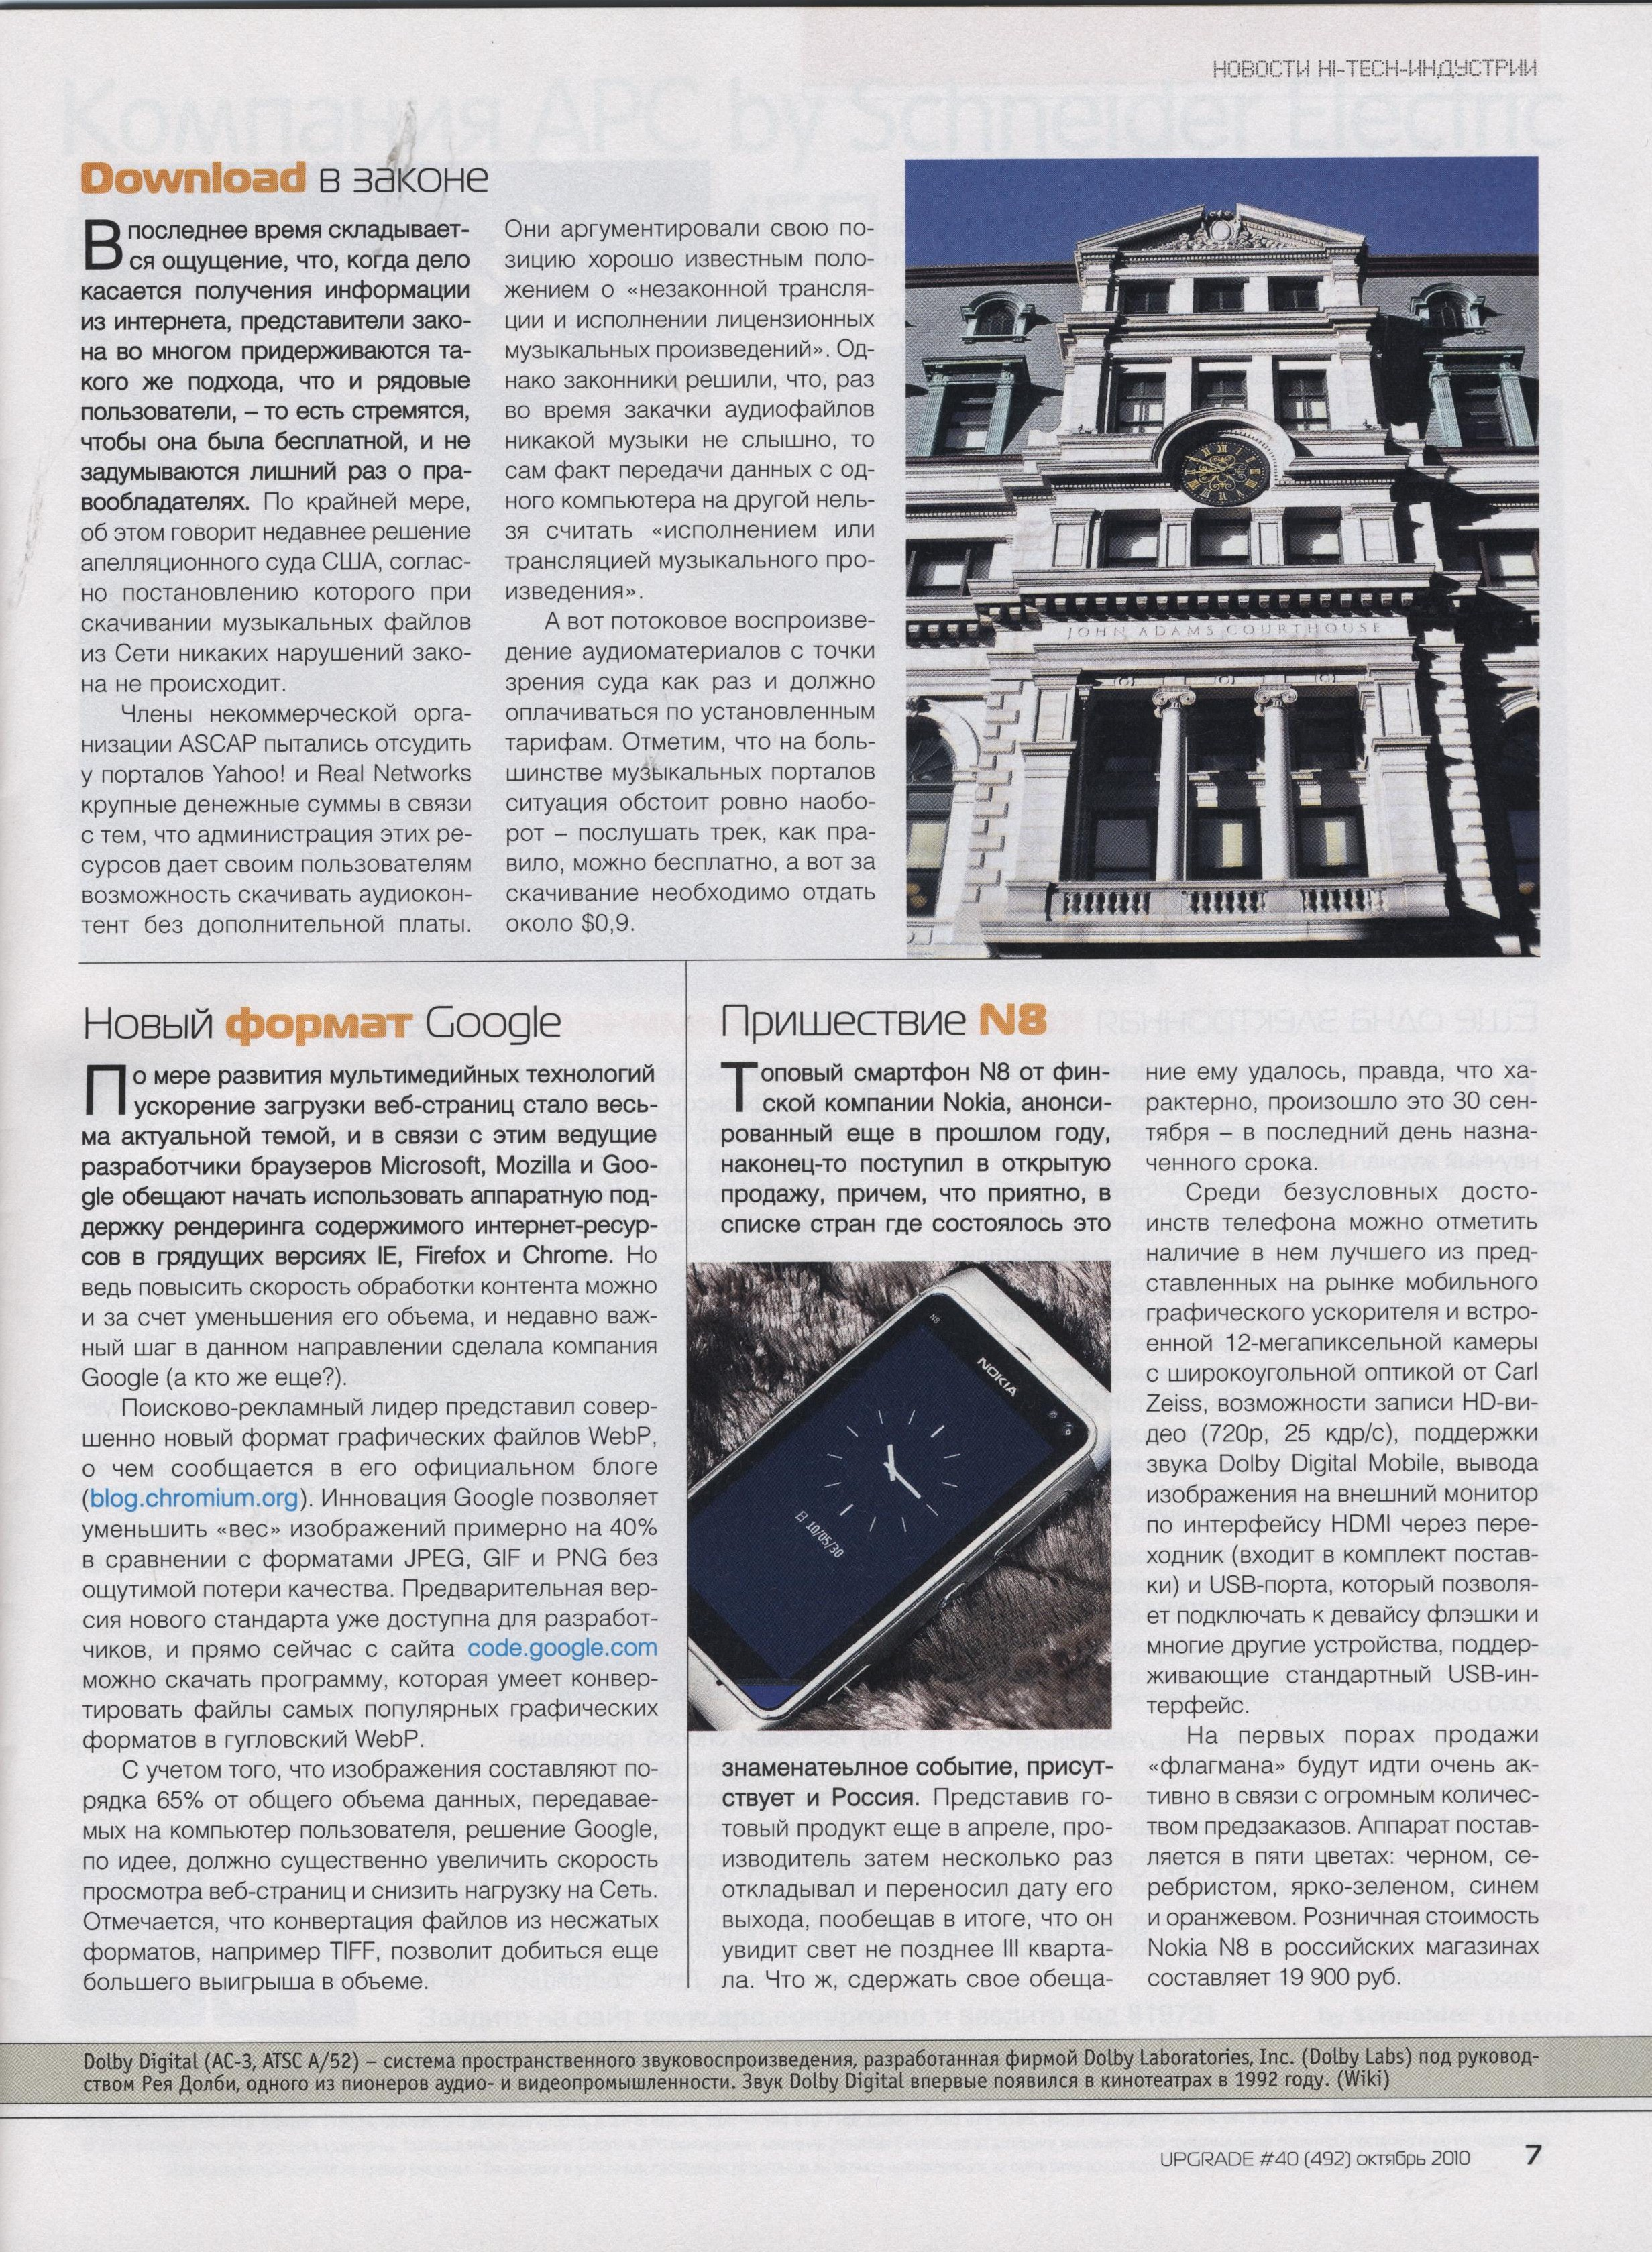
\includegraphics[scale=0.2]{images/4.jpg}
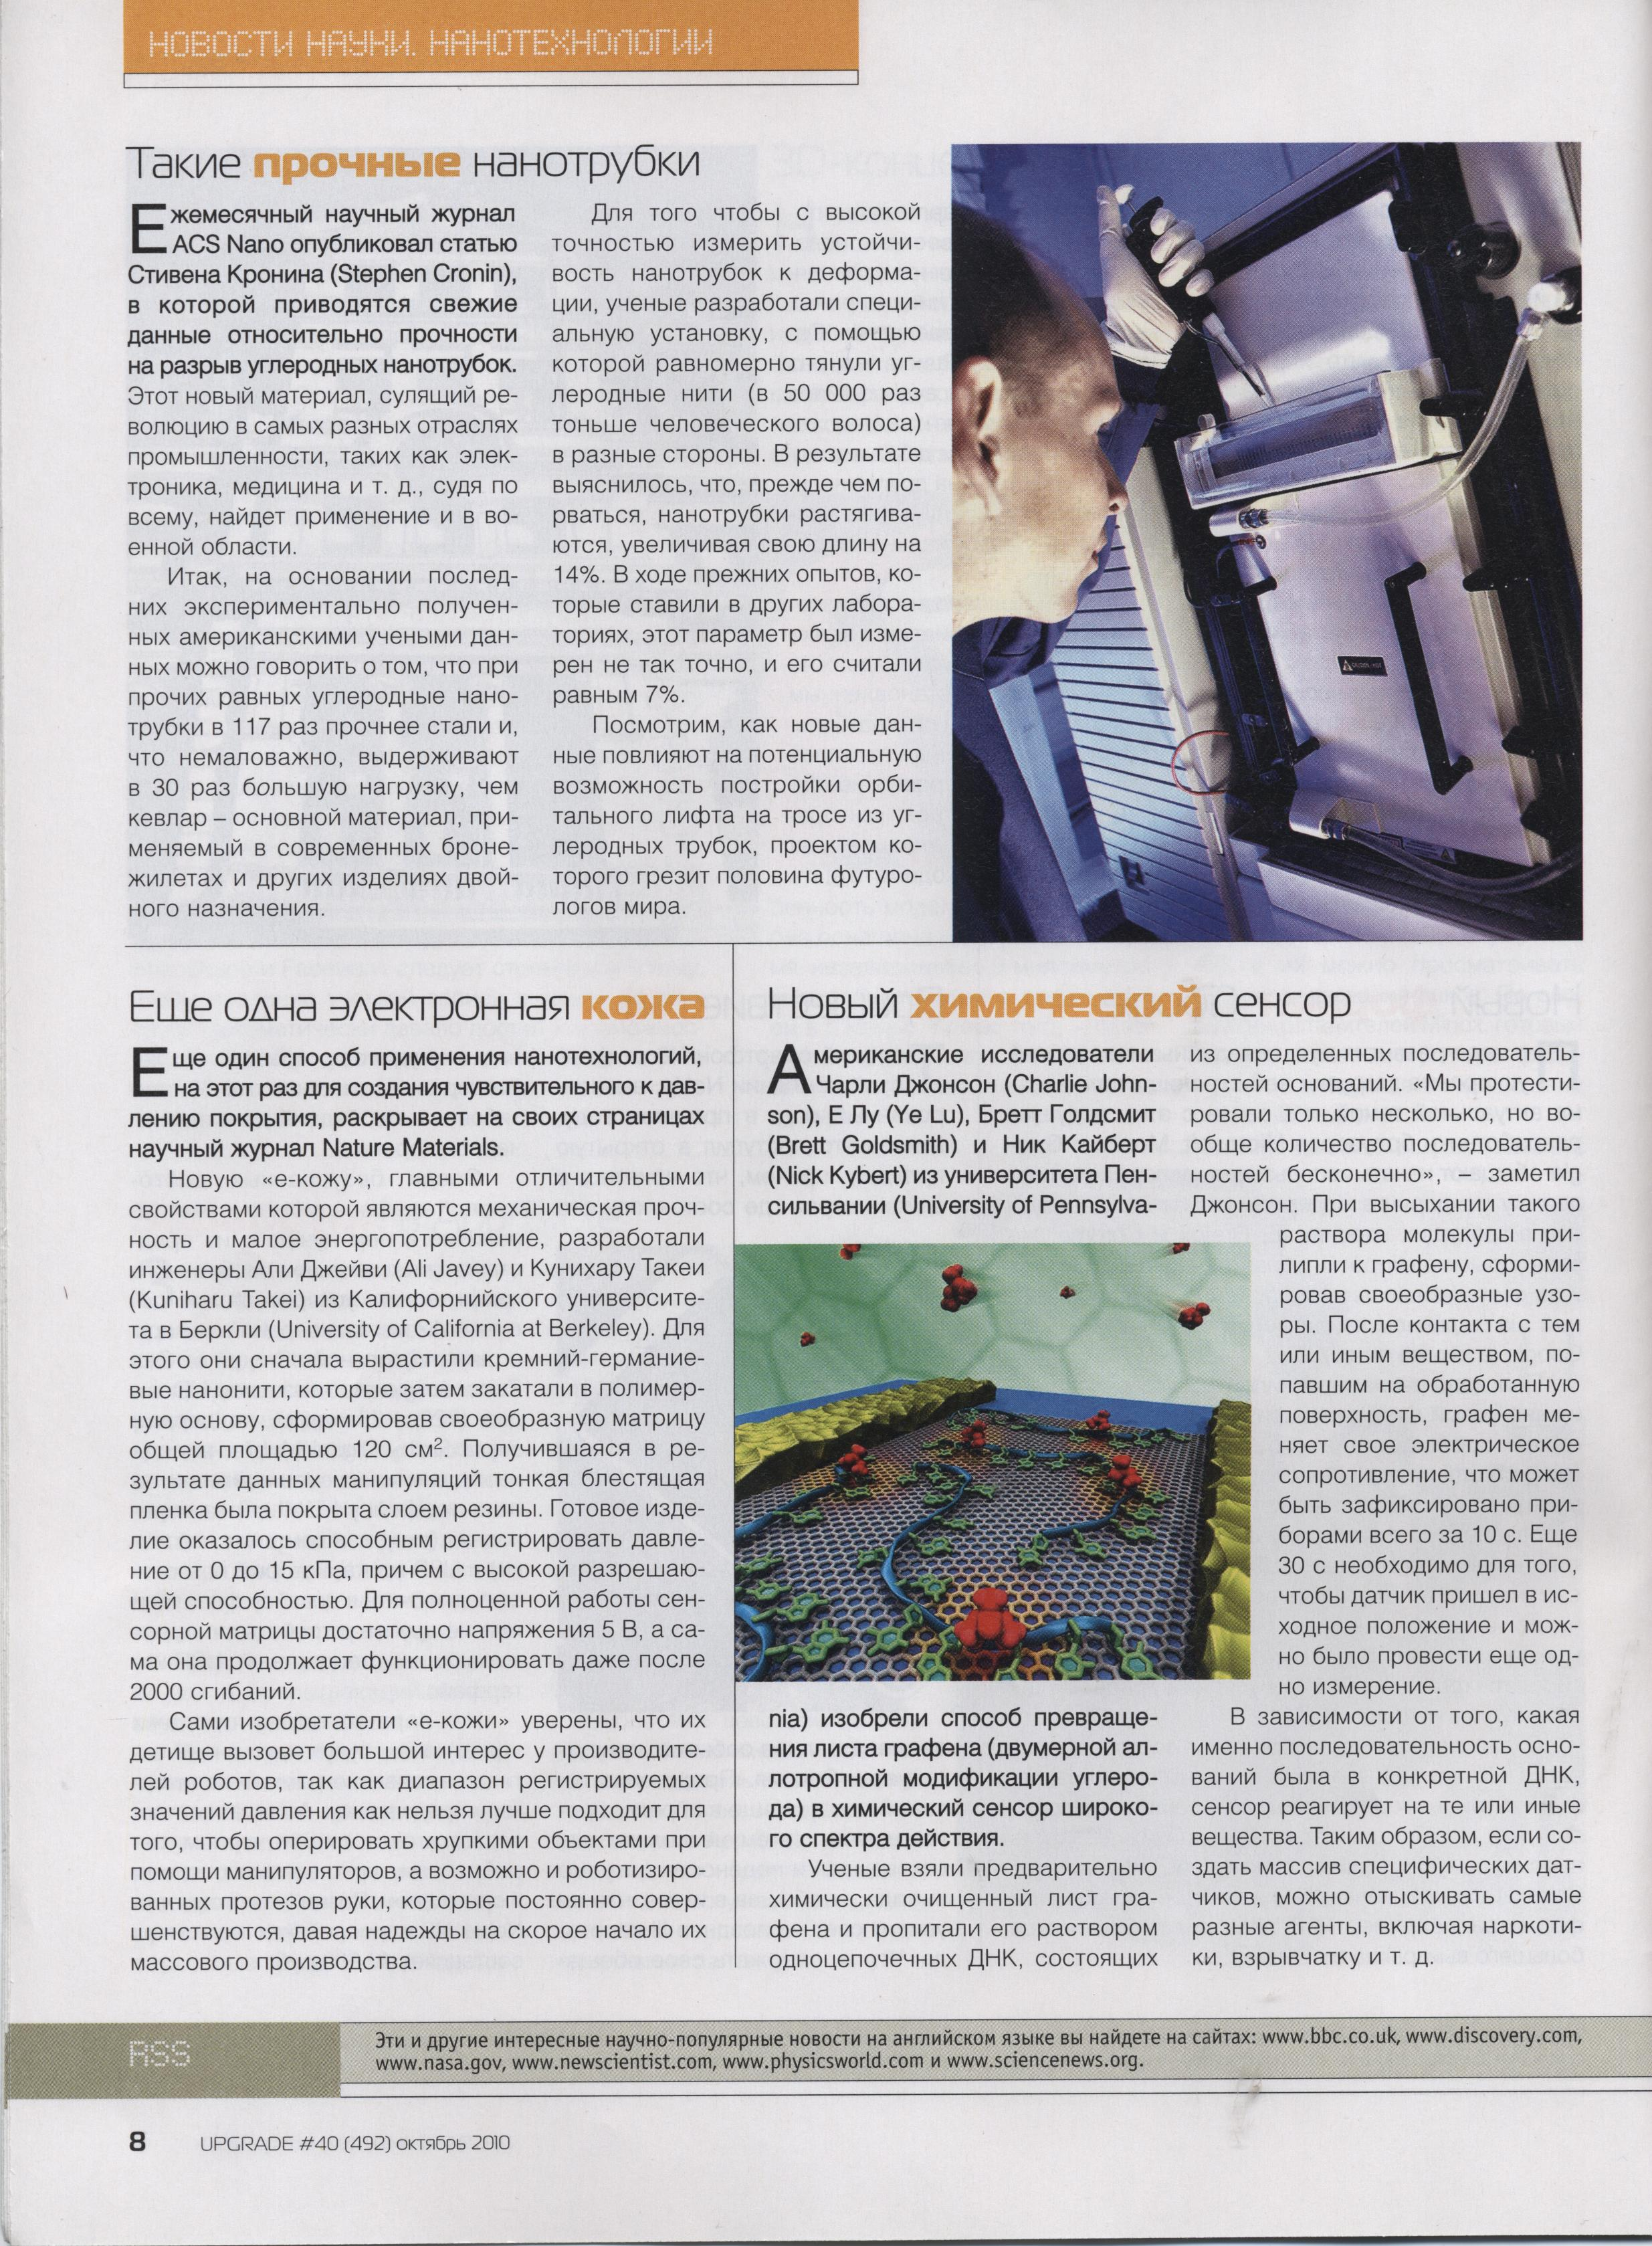
\includegraphics[scale=0.2]{images/5.jpg}
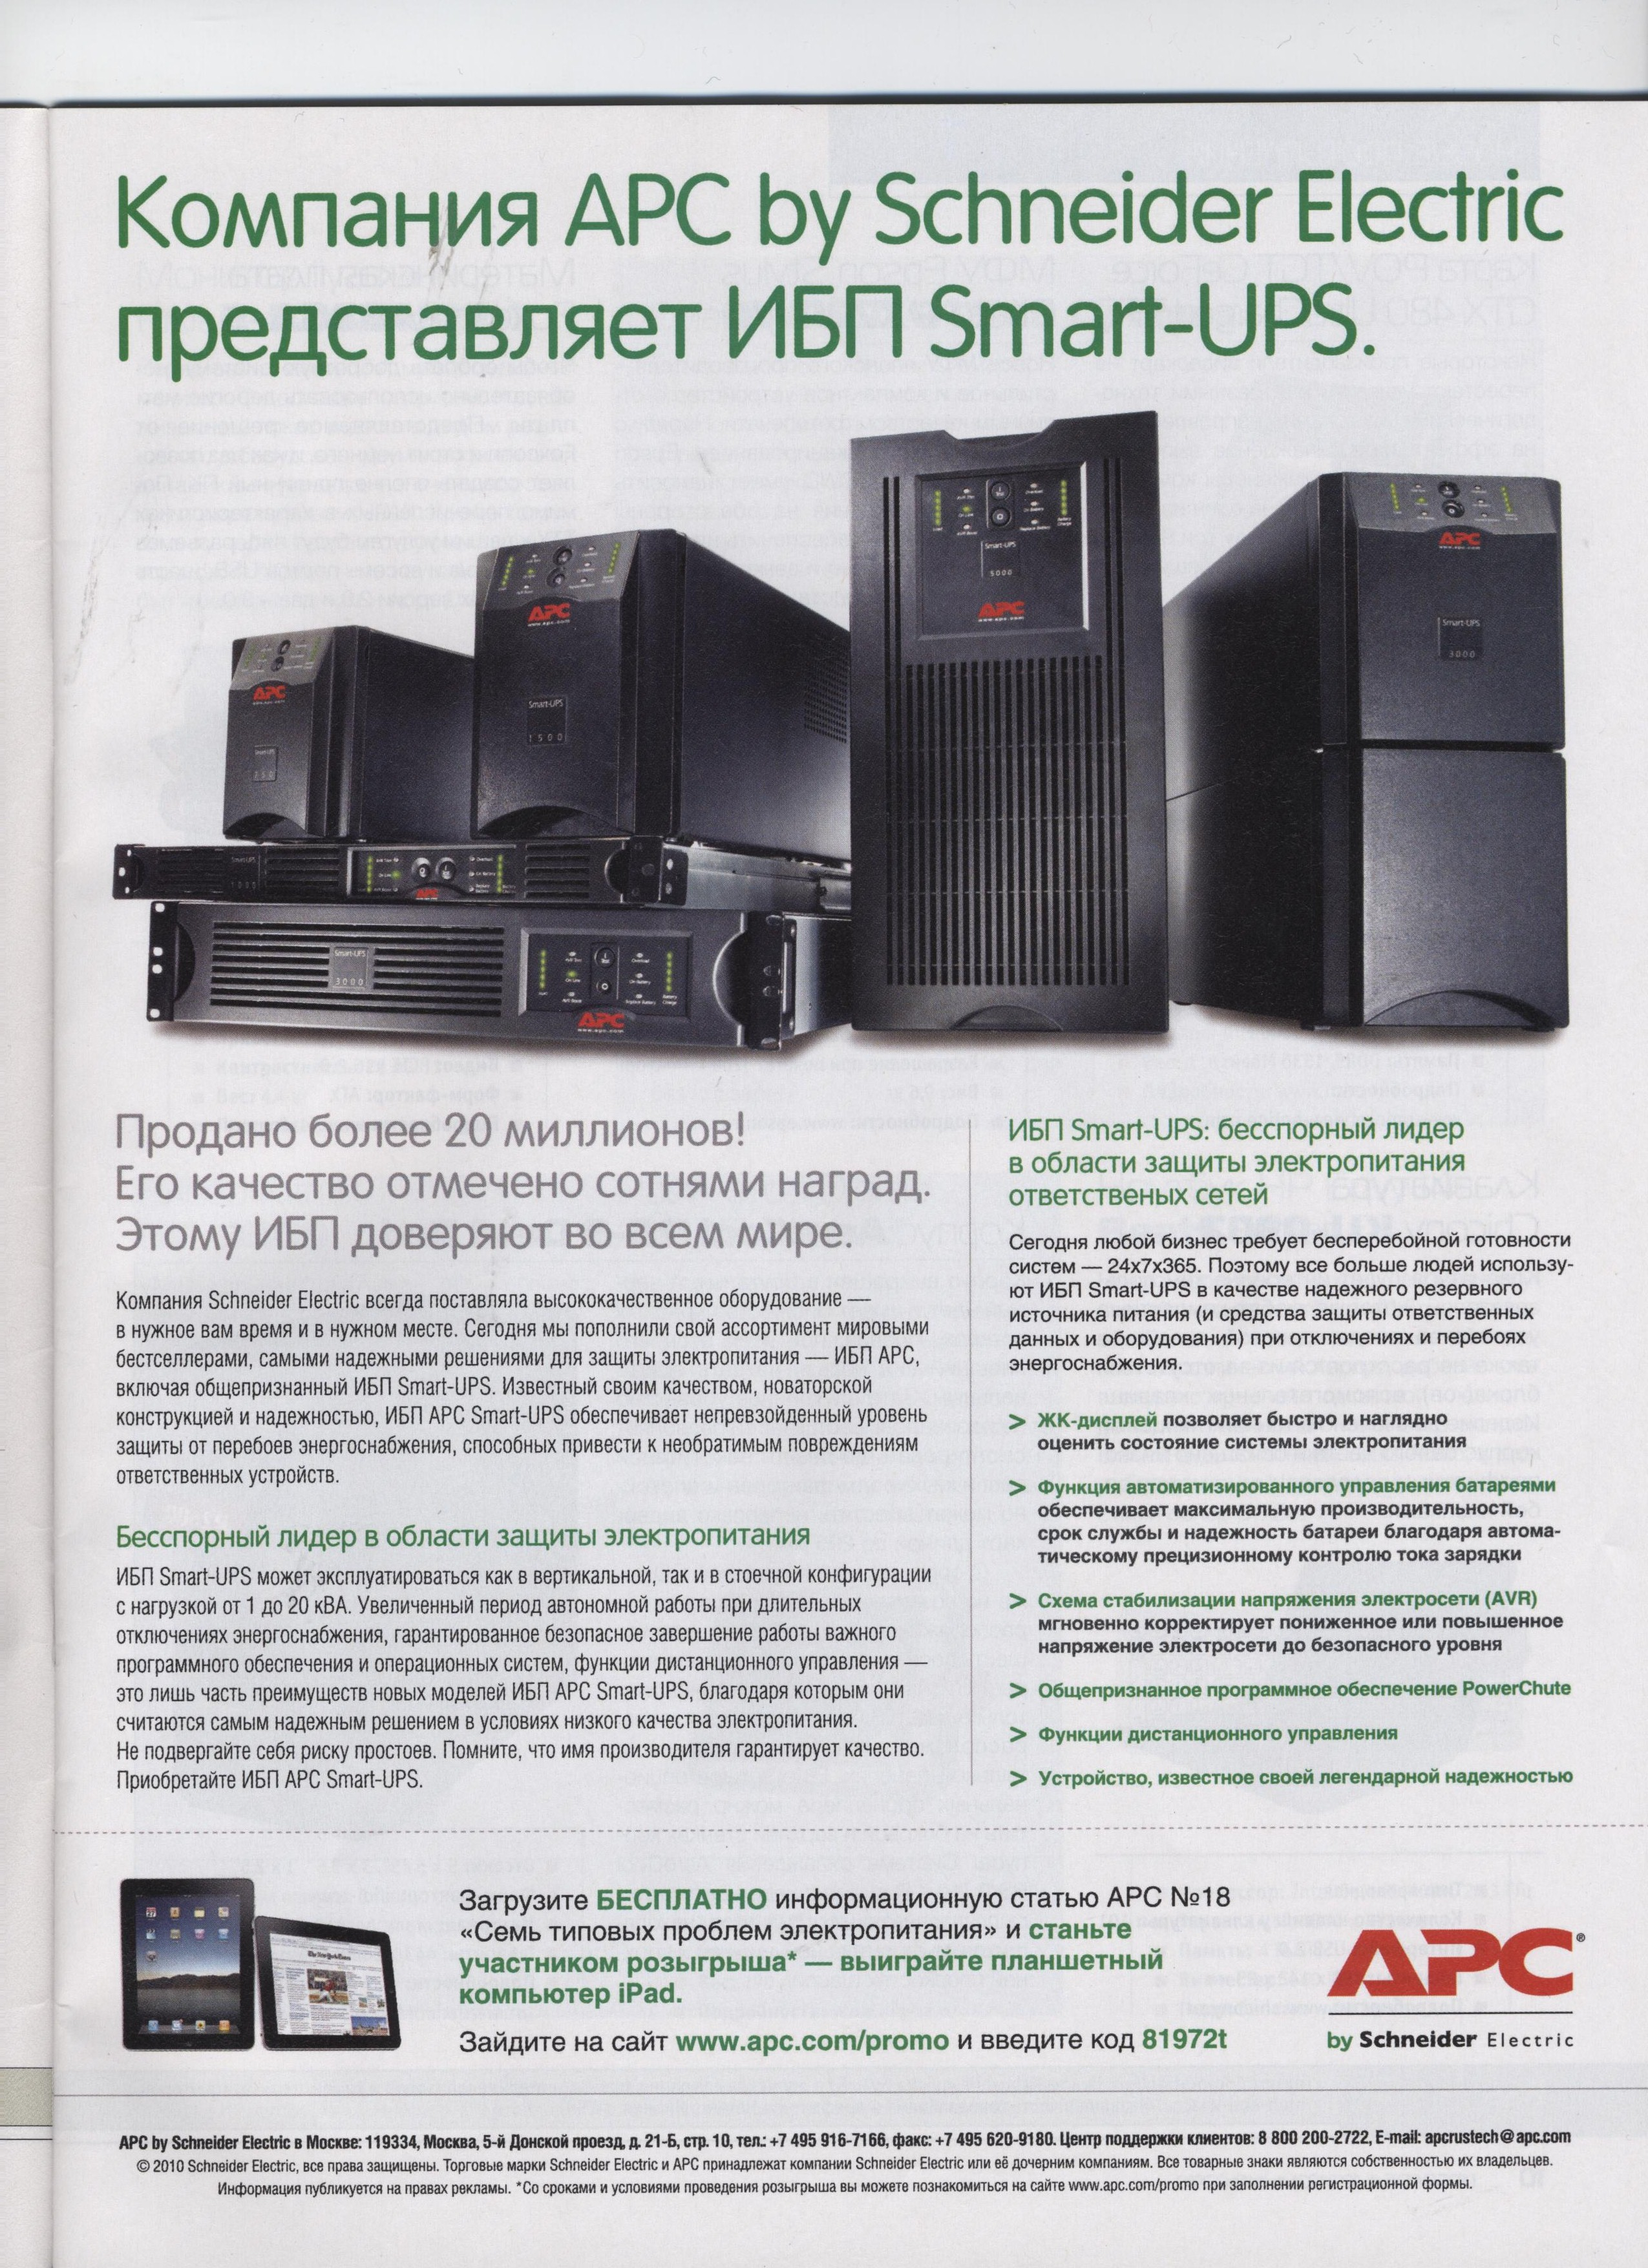
\includegraphics[scale=0.2]{images/6.jpg}
\end{center}
\caption{Exemples d'images du dataset}
\label{exemple1}
\end{figure}
\clearpage

\section{Vérité-terrain}
A chacune de ces images est associée une image de vérite-terrain, attribuant à chaque pixel du document numérisé l'une des 3 classes parmi : \\
\begin{description} % listes descriptives

\item[$illustration$ :] Le pixel appartient à une illustration, une image, un fond d'image, un logo (en rouge sur les images vérité-terrain)
\item[$texte$ :] Le pixel appartient à un paragraphe de texte, un titre, un commentaire (en bleu sur les images vérité-terrain)
\item[$fond$ :] Le pixel appartient au fond blanc d'origine de la page (en blanc sur les images vérité-terrain).

\end{description}

Voici quelques exemples de documents numérisés et leur vérité terrain \ref{exemple1} \ref{exemple2} \ref{exemple3}.

\begin{figure}[H]
\begin{center}
\includegraphics[scale=0.2]{images/1g.jpg}
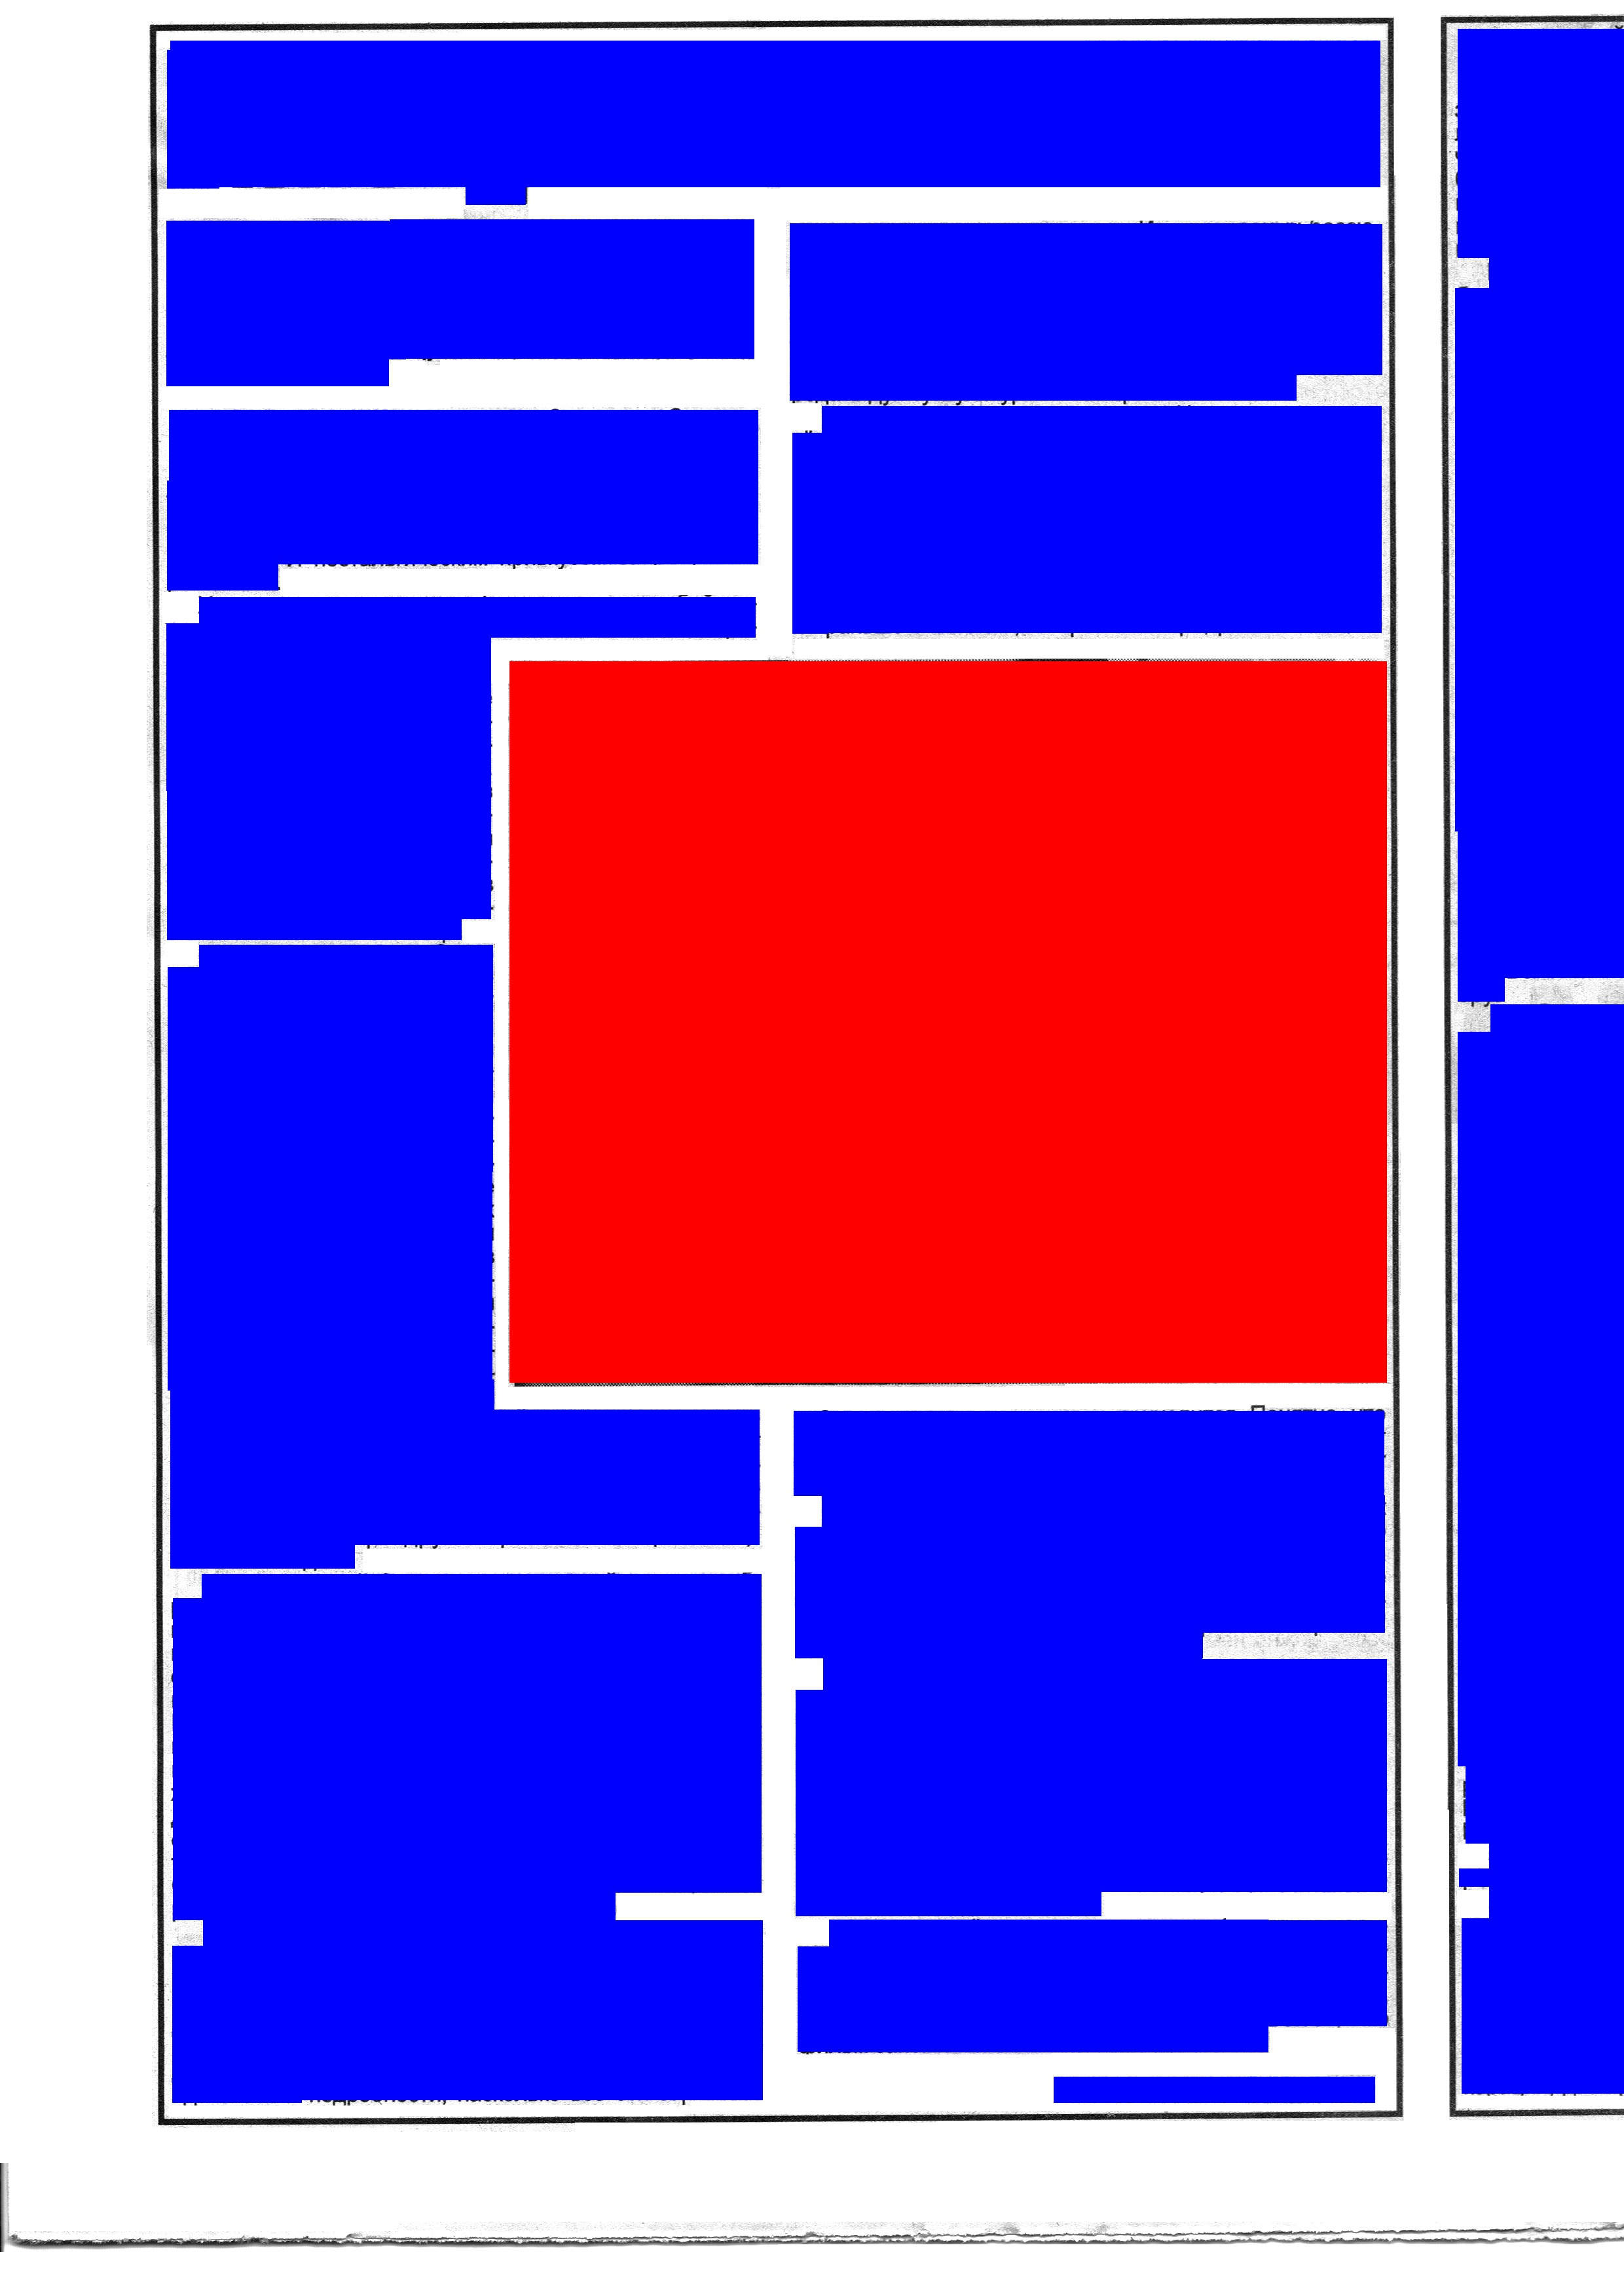
\includegraphics[scale=0.2]{images/1g_m.jpg}
\end{center}
\caption{image du dataset et sa vérité terrain}
\label{exemple1}
\end{figure}

\begin{figure}[H]
\begin{center}
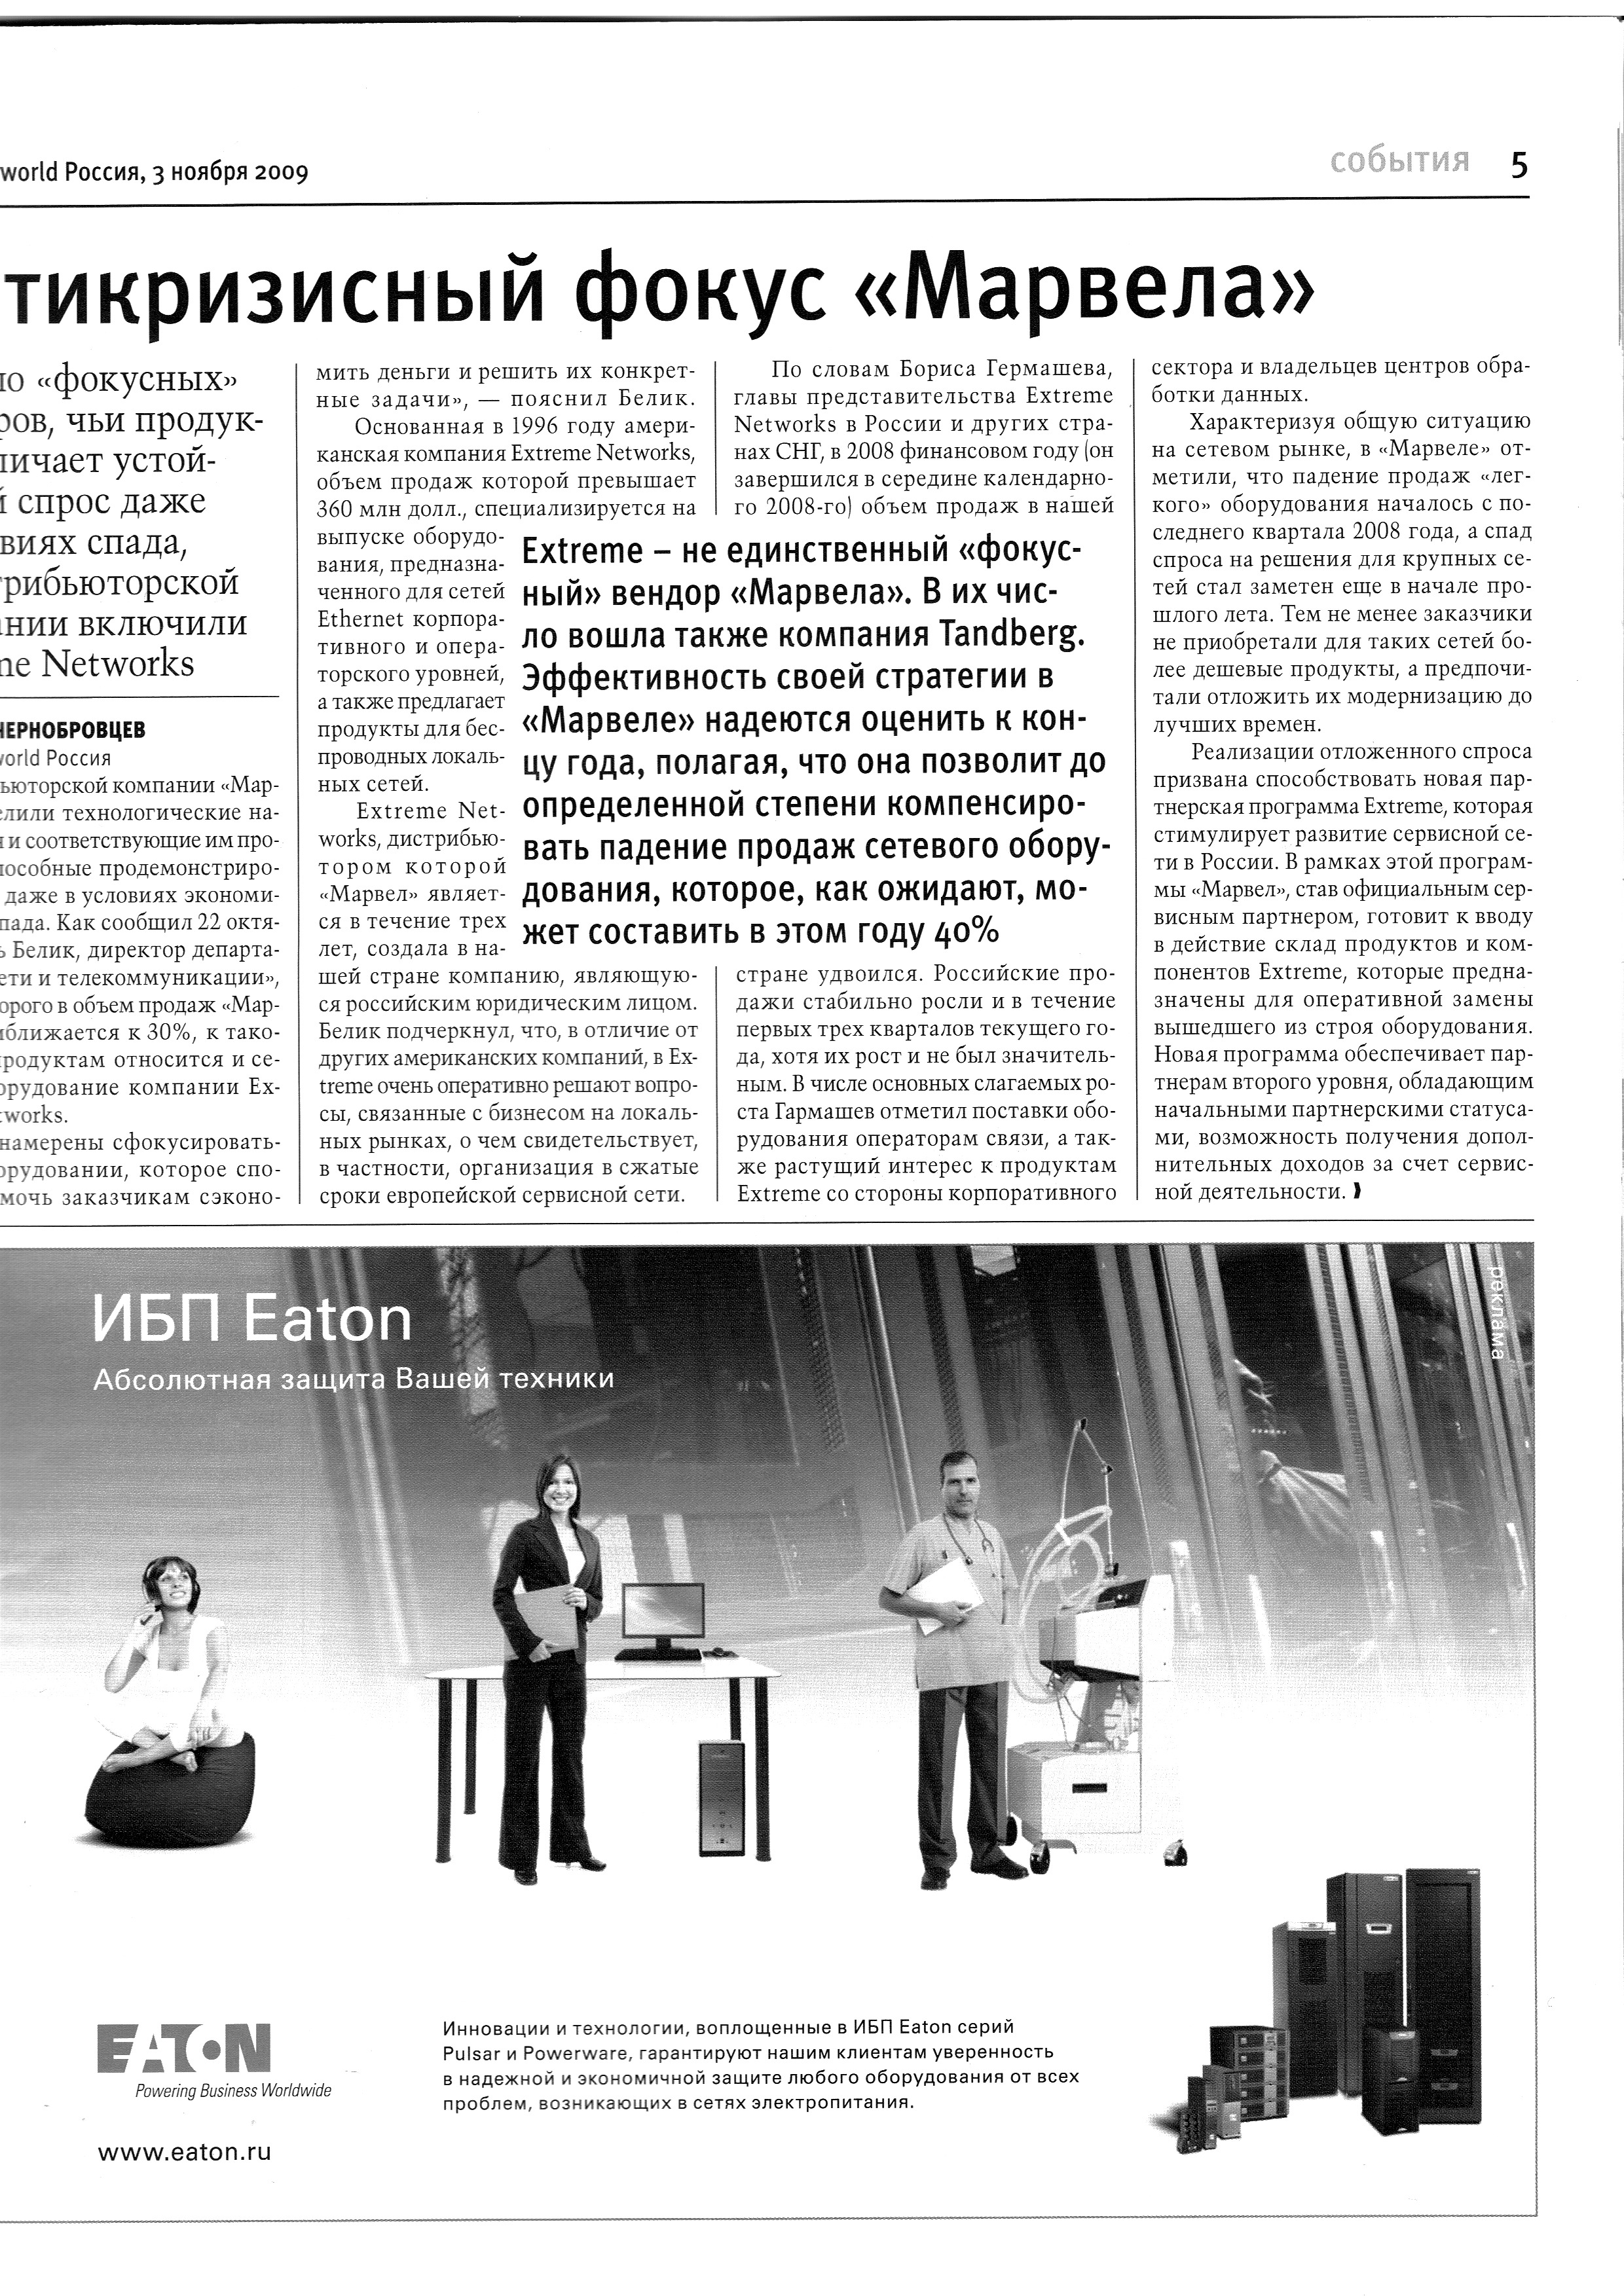
\includegraphics[scale=0.2]{images/4cw.jpg}
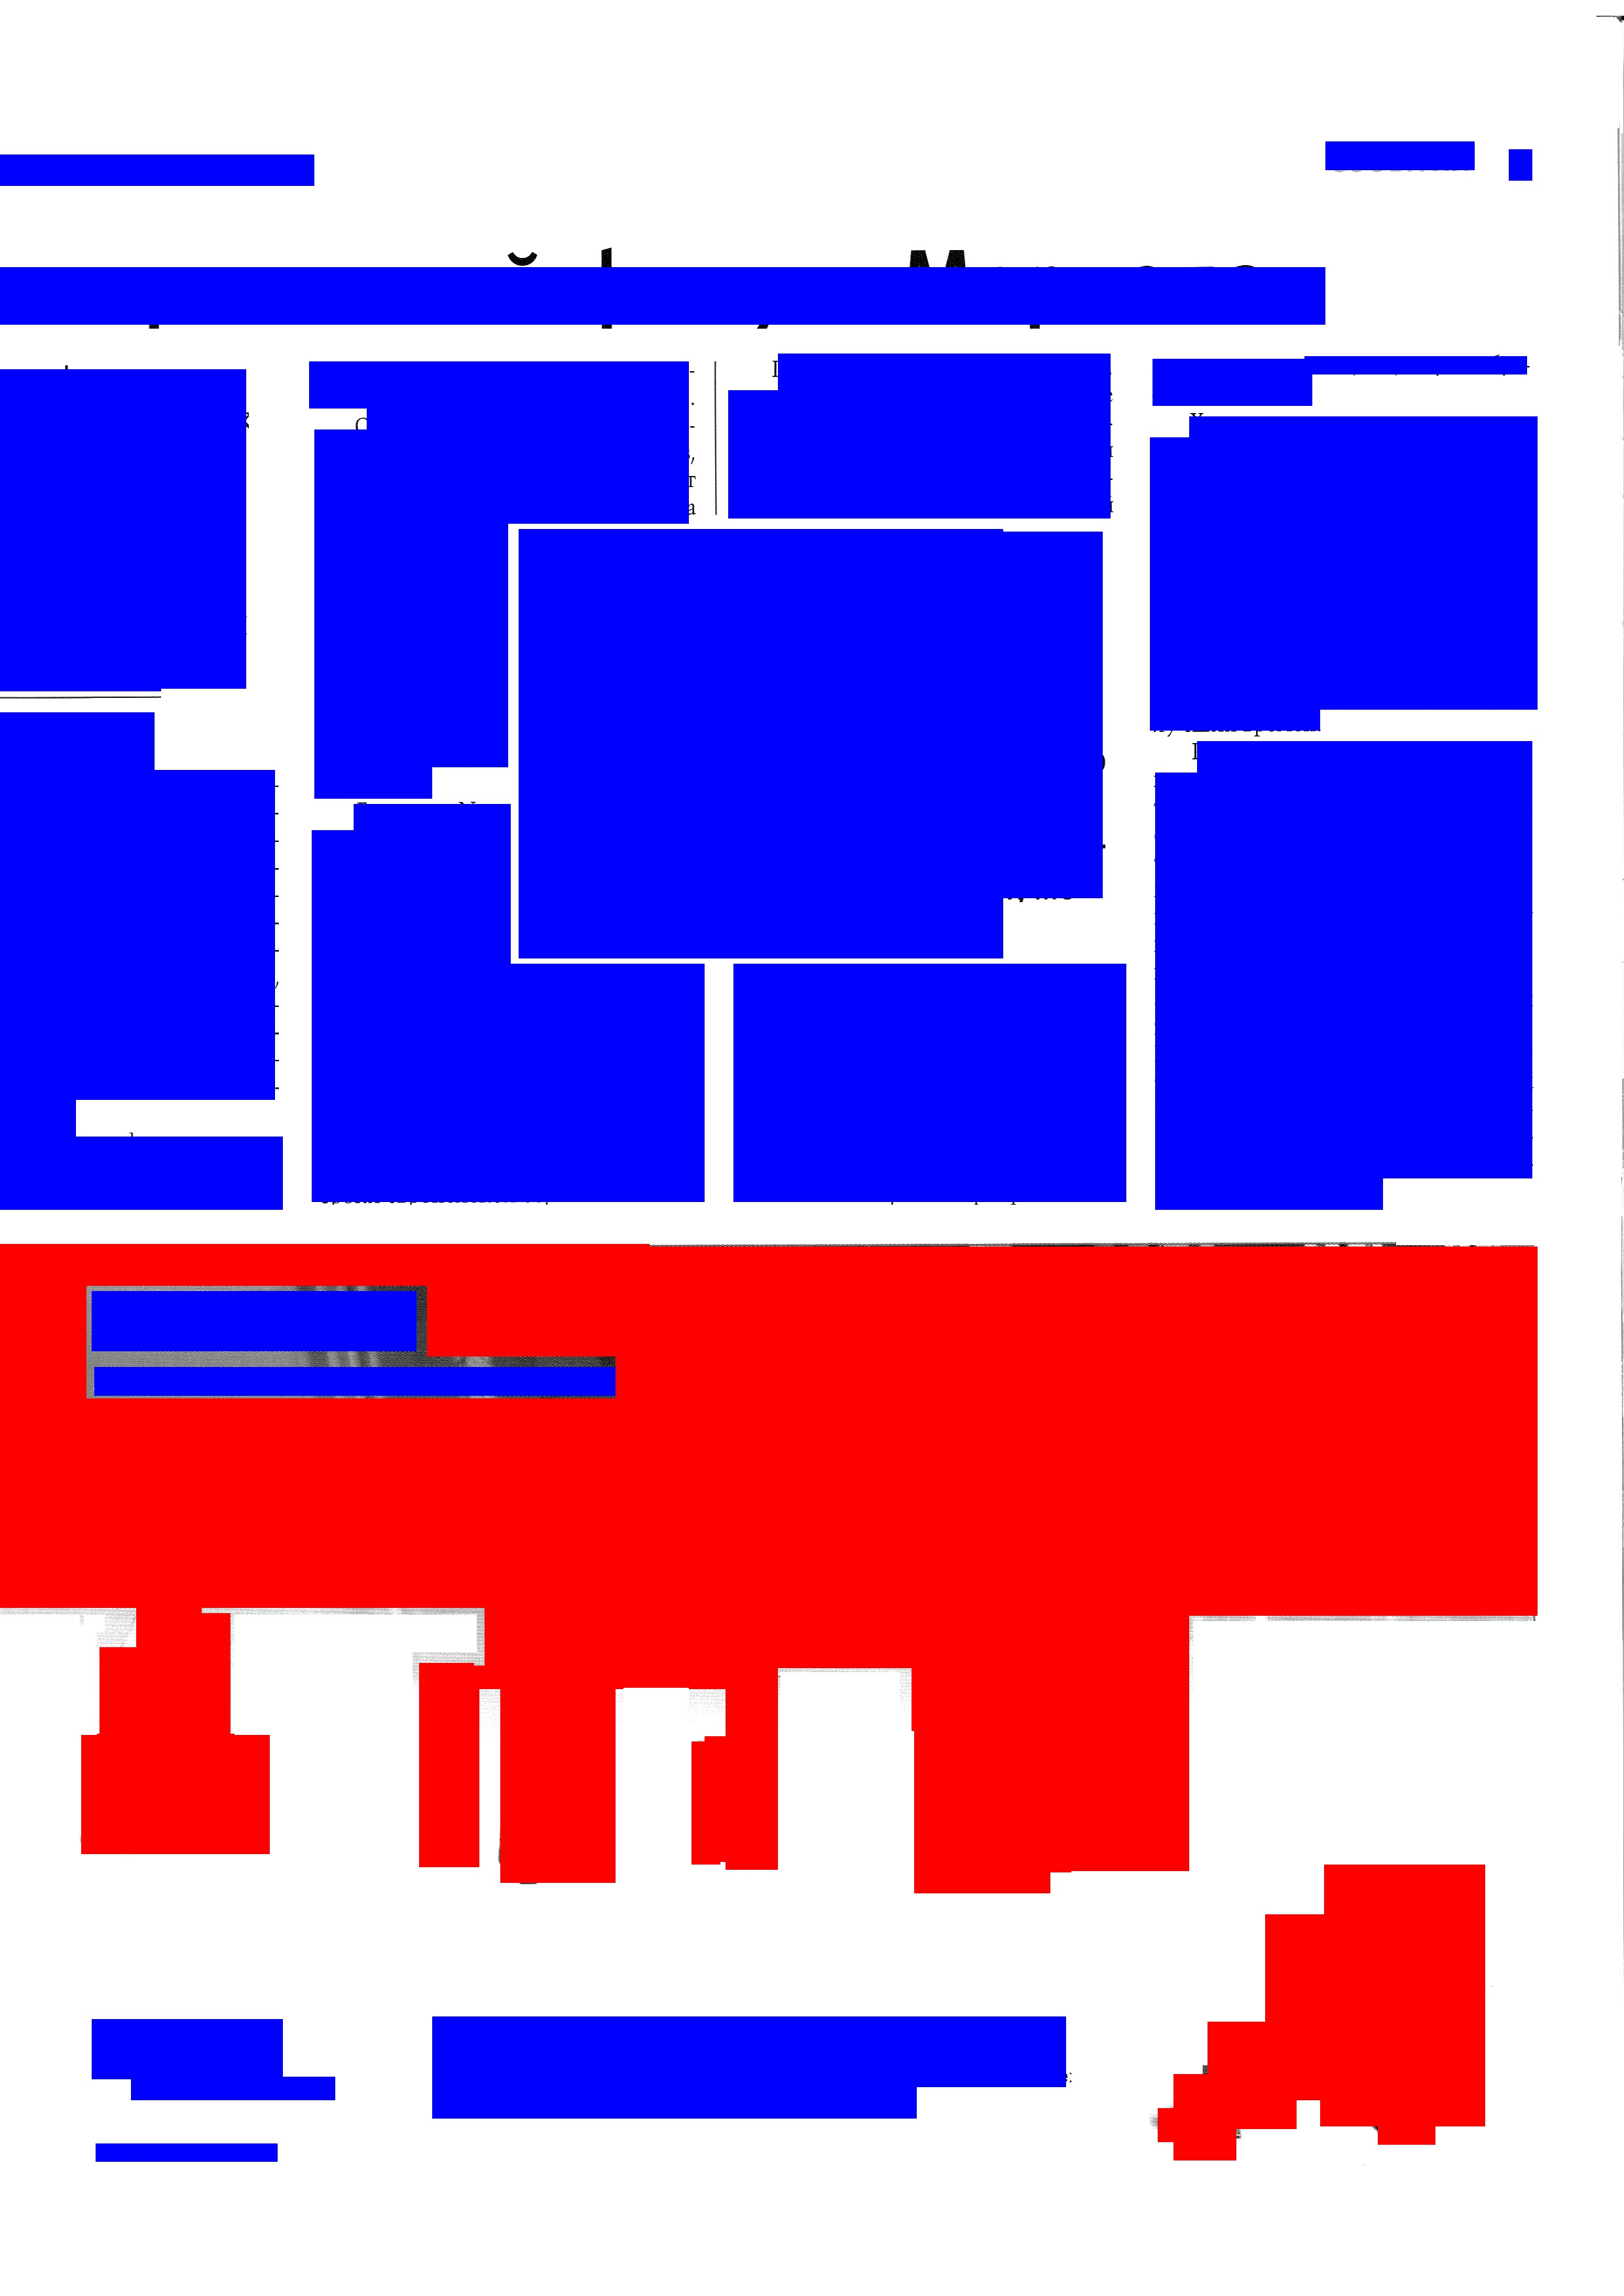
\includegraphics[scale=0.2]{images/4cw_m.jpg}
\end{center}
\caption{image du dataset et sa vérité terrain}
\label{exemple2}
\end{figure}

\begin{figure}[H]
\begin{center}

\includegraphics[scale=0.2]{images/56.jpg}

\includegraphics[scale=0.2]{images/56_m.jpg}
\end{center}
\caption{image du dataset et sa vérité terrain}
\label{exemple3}
\end{figure}
\clearpage

Par la suite, nous allons expliciter différentes manières d'extraire de l'information afin de pouvoir discriminer automatiquement, au sein d'une image, les pixels de classe
$illustration$, de classe $texte$ et de classe $fond$.

\chapter{Extraction d'information}
\section{Seuillage pour le fond}

Une manière simple et rapide d'isoler le fond, est de réaliser un seuillage de l'image passée en niveau de gris.\\
Le seuil d'Otsu cherche le seuil qui sépare l'histogramme des niveaux de gris en deux classes, de sorte que la variance inter-classe soit maximale, la variance intra-classe
minimale \ref{seuillage}.\\

\begin{figure}[H]
\begin{center}
\includegraphics[scale=0.2]{images/1g.jpg}
%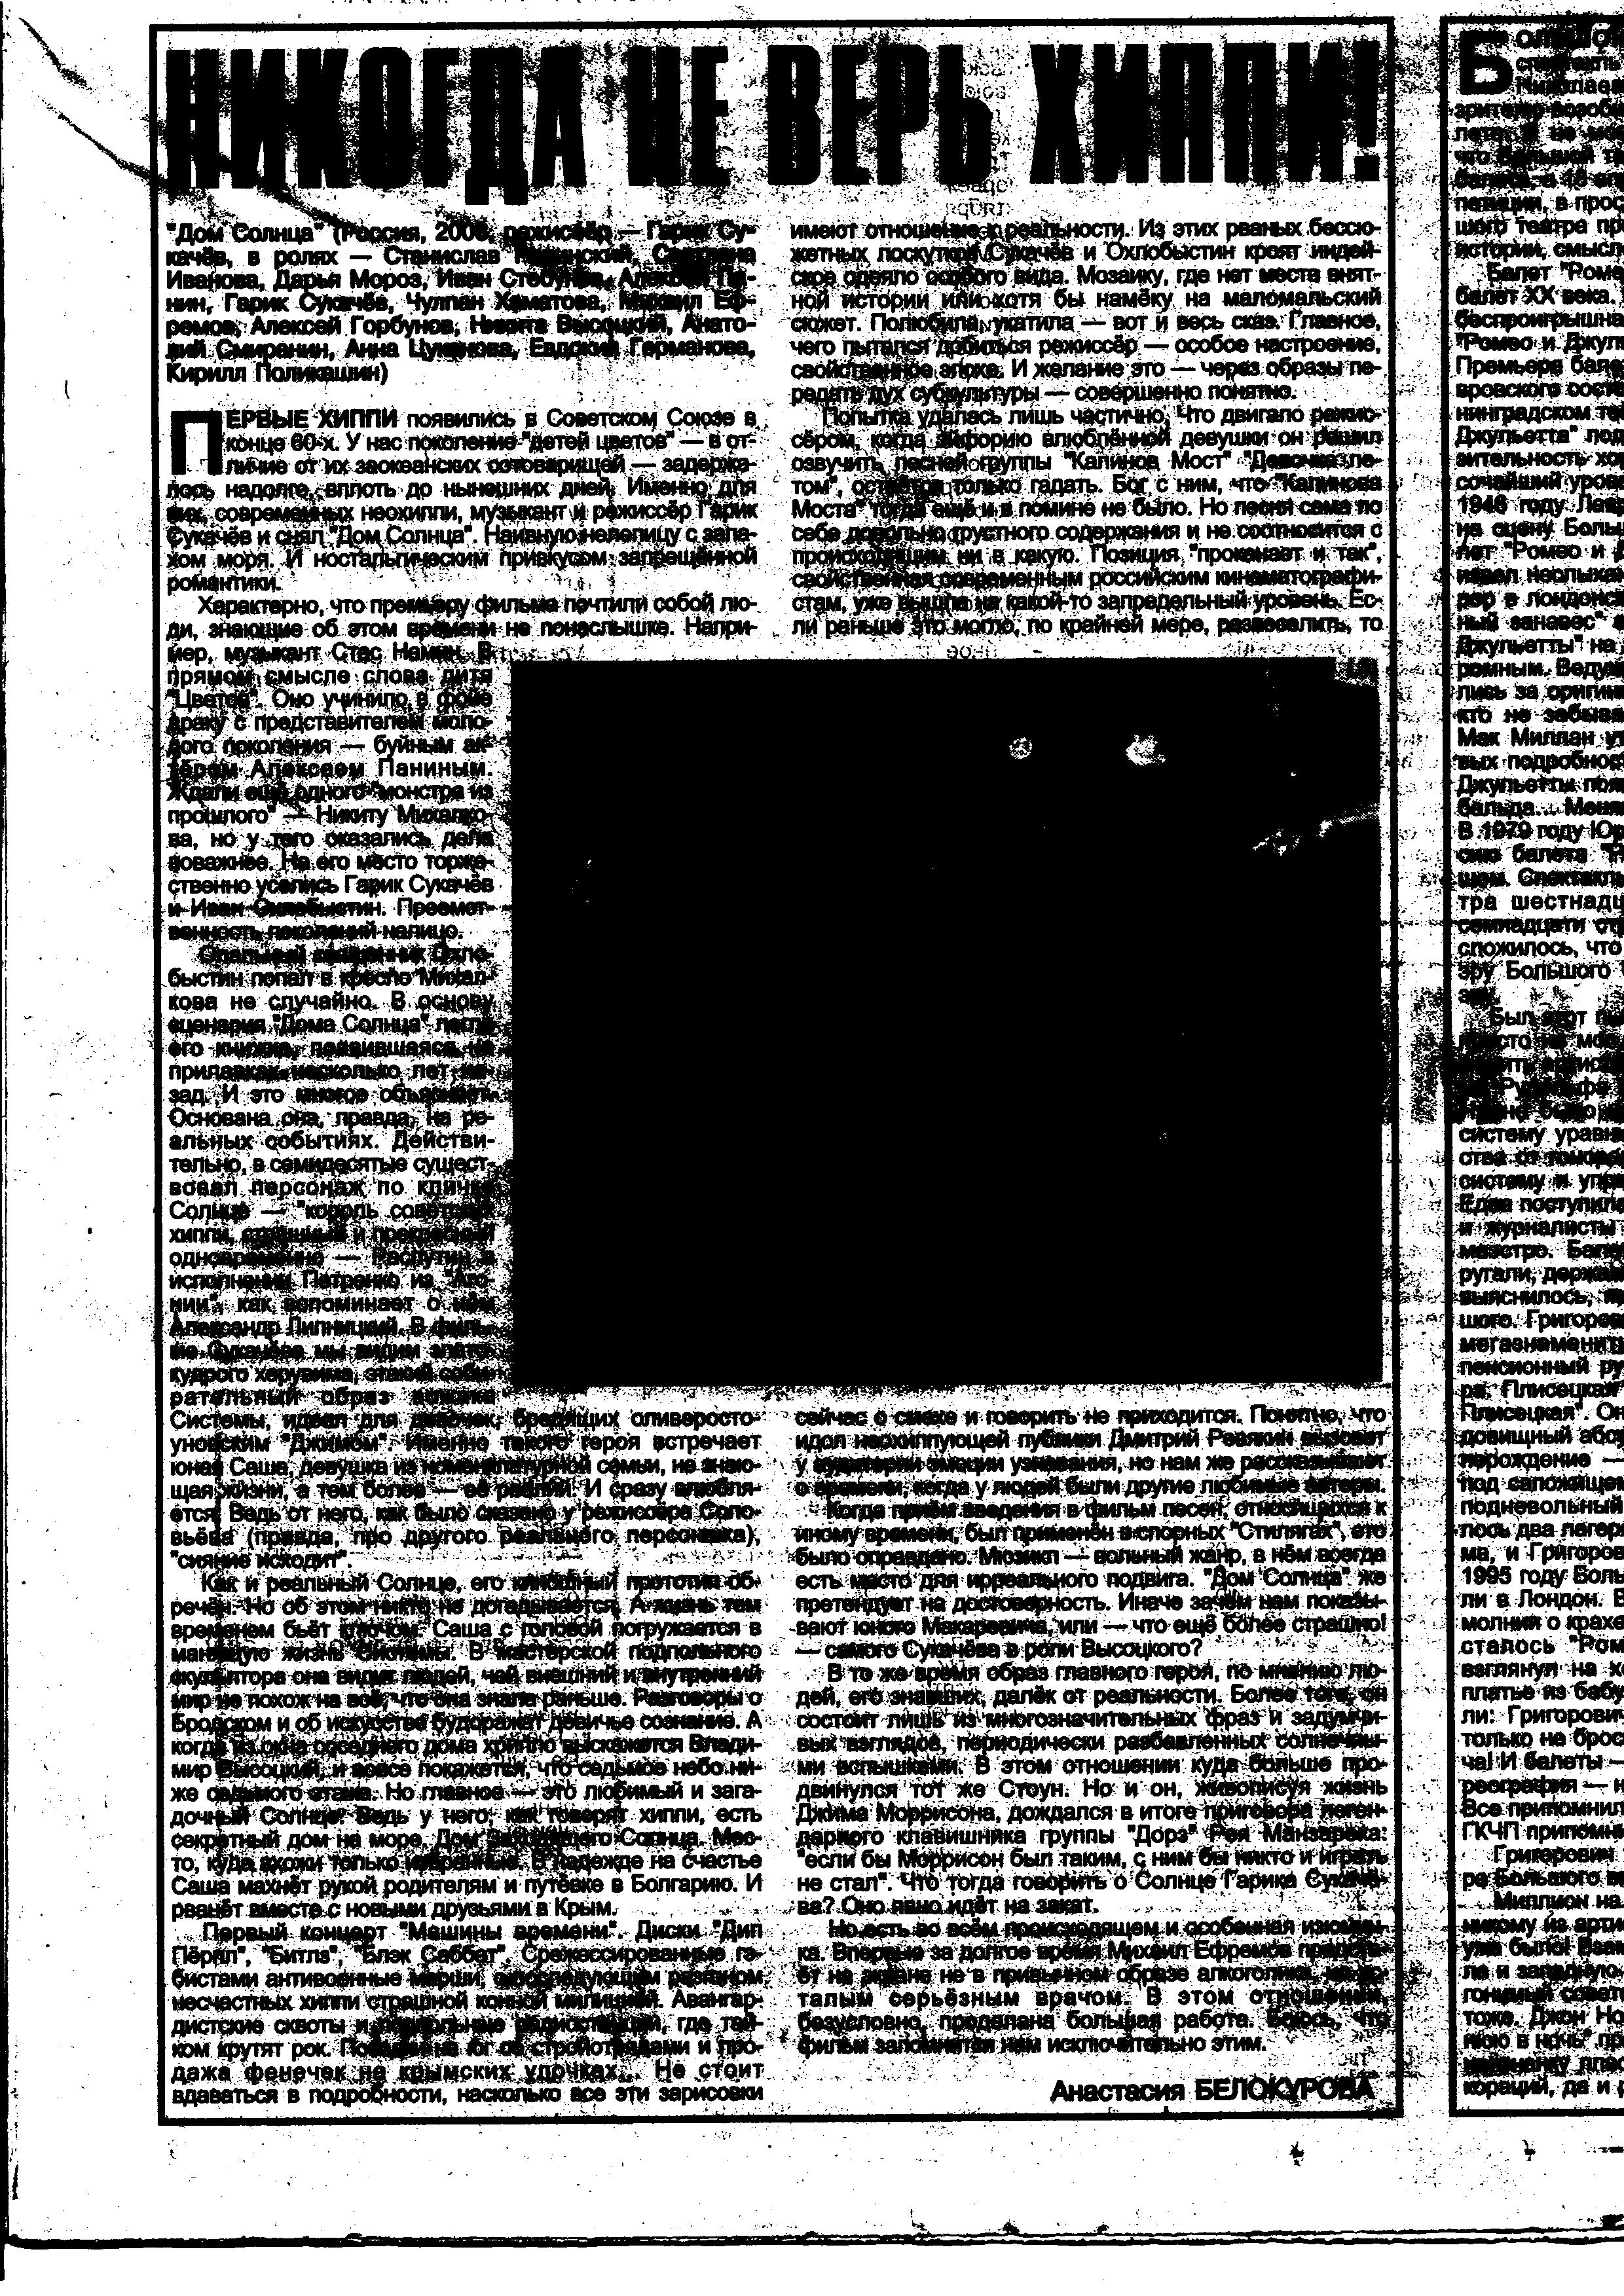
\includegraphics[scale=0.2]{images/1g_binary.jpg}
\end{center}
\caption{seuillage}
\label{seuillage}
\end{figure}

Ainsi, cette première étape permet de trouver les pixels de $fond$. En effet, on attribue une telle classe aux pixels dont le voisinage carré est à 95\% blanc 
dans l'image binaire.

\begin{figure}[H]
\begin{center}
%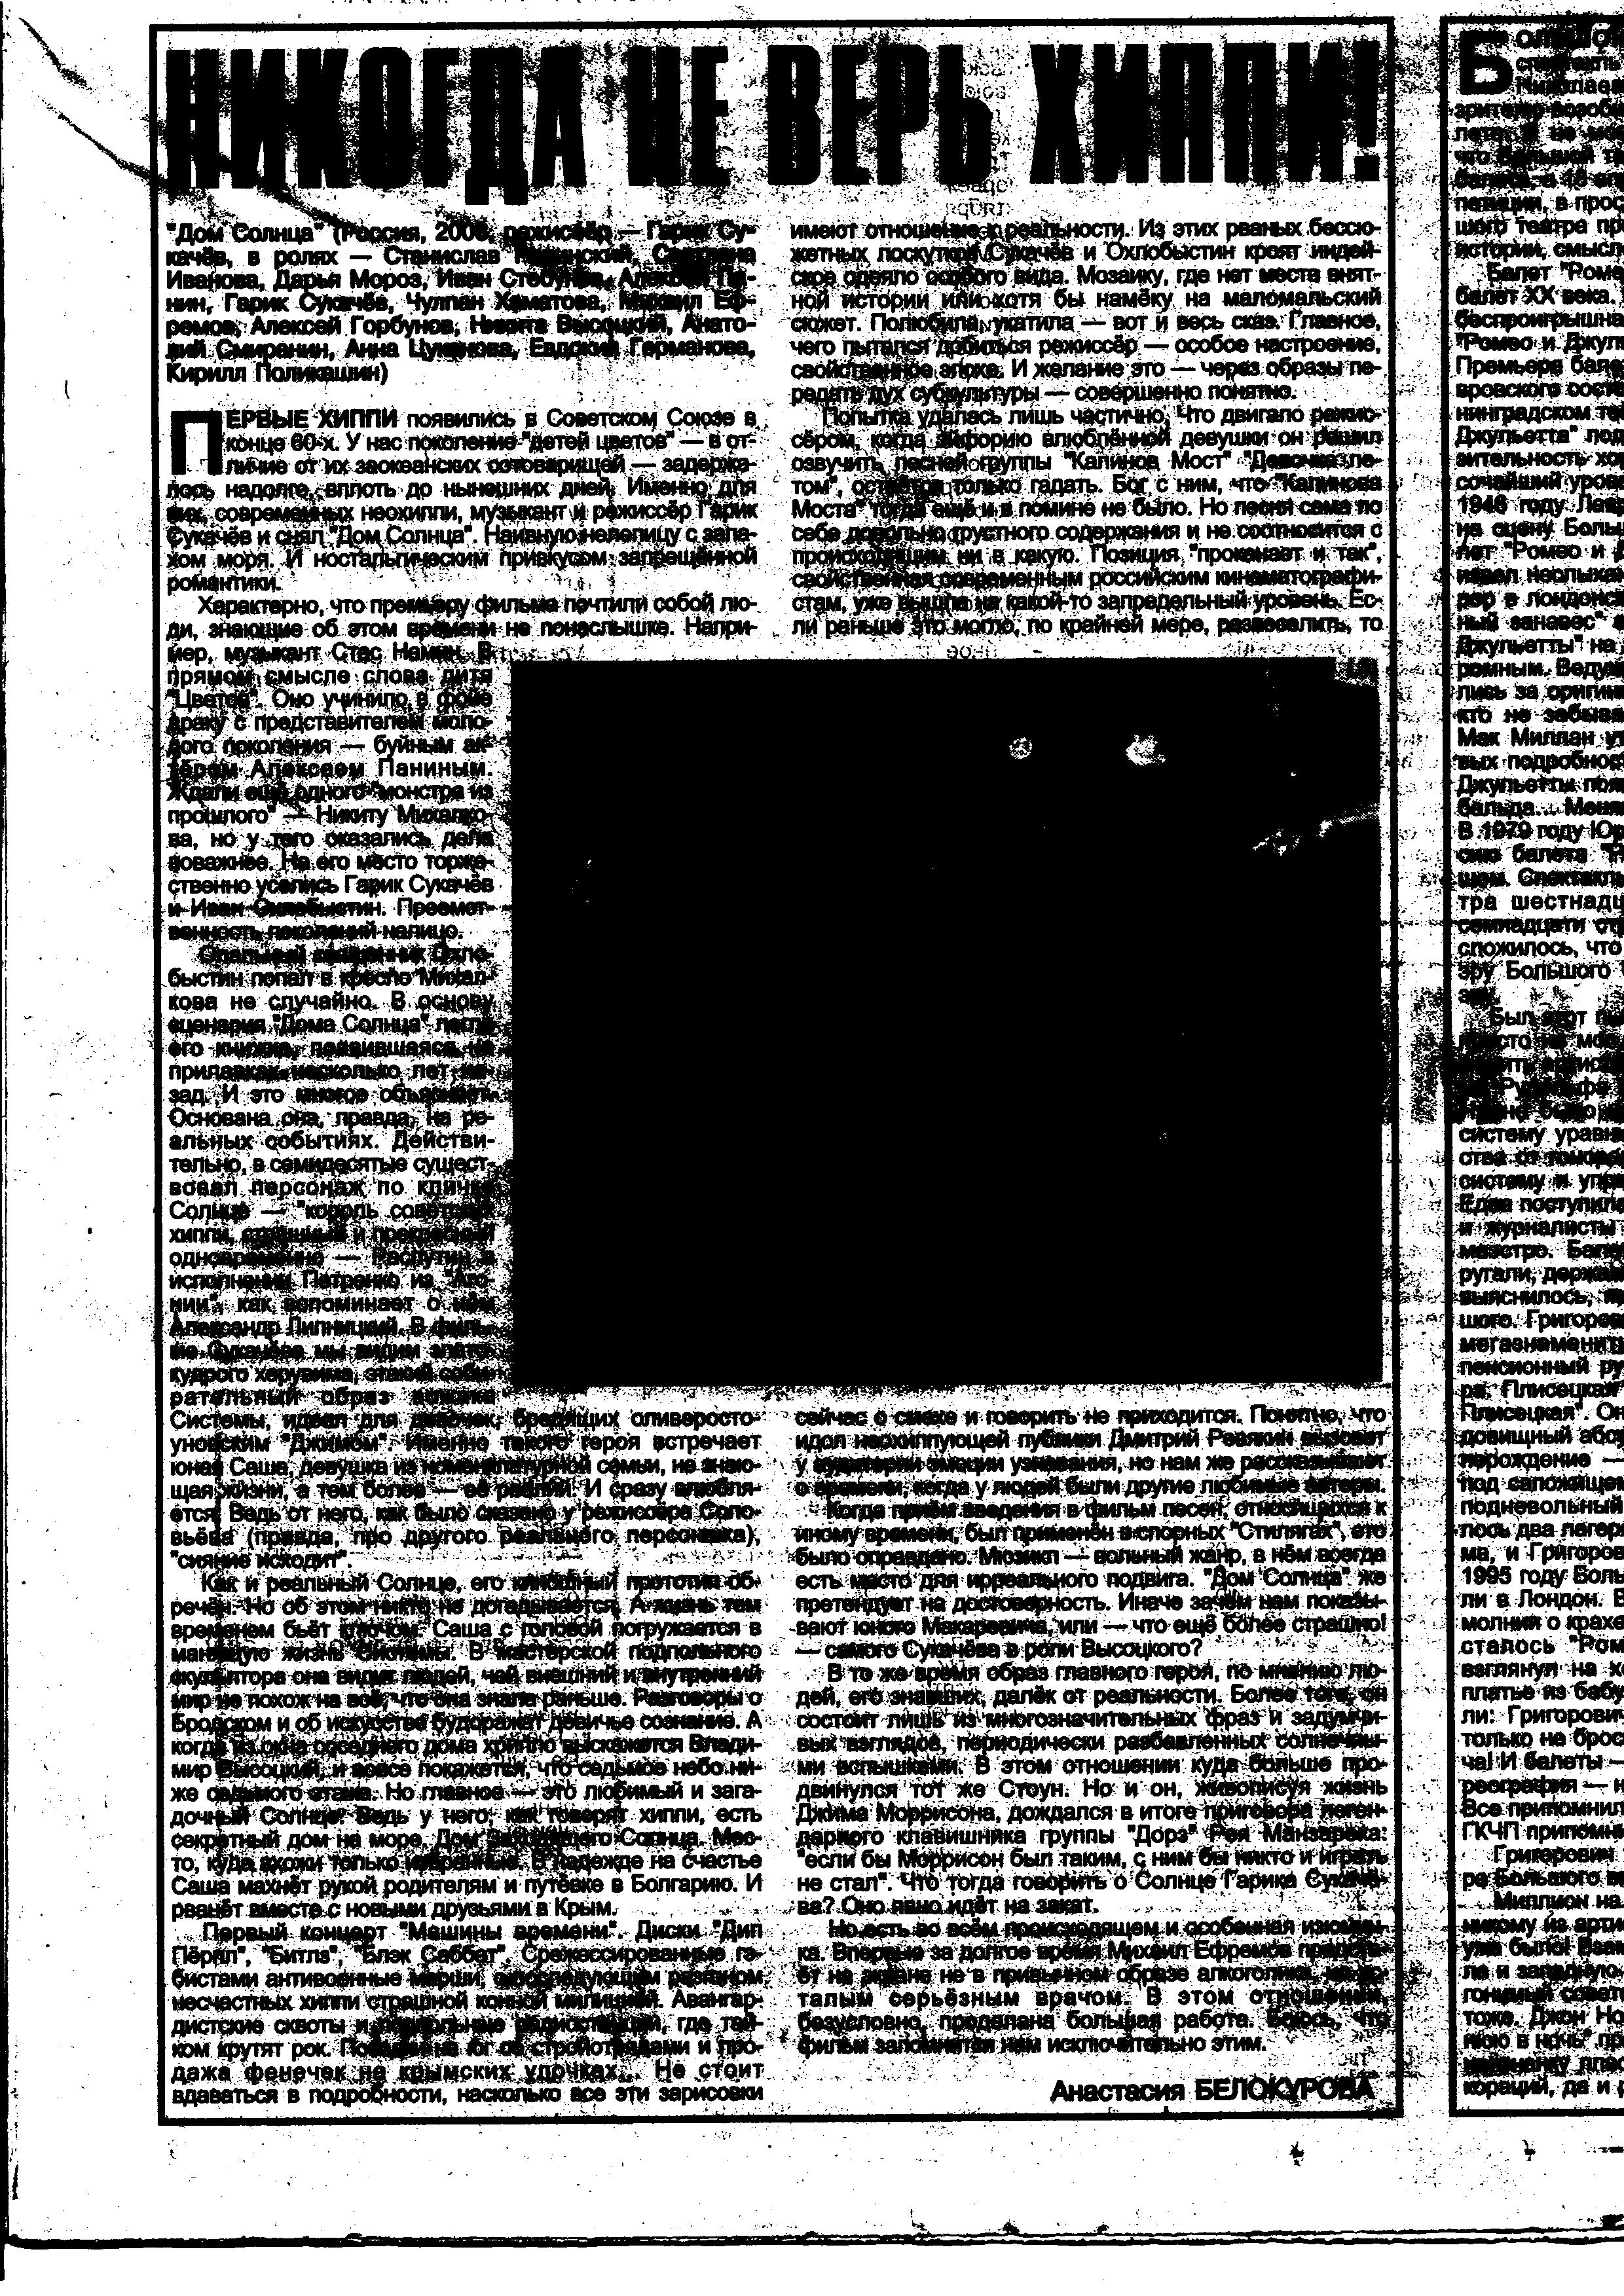
\includegraphics[scale=0.2]{images/1g_binary.jpg}
%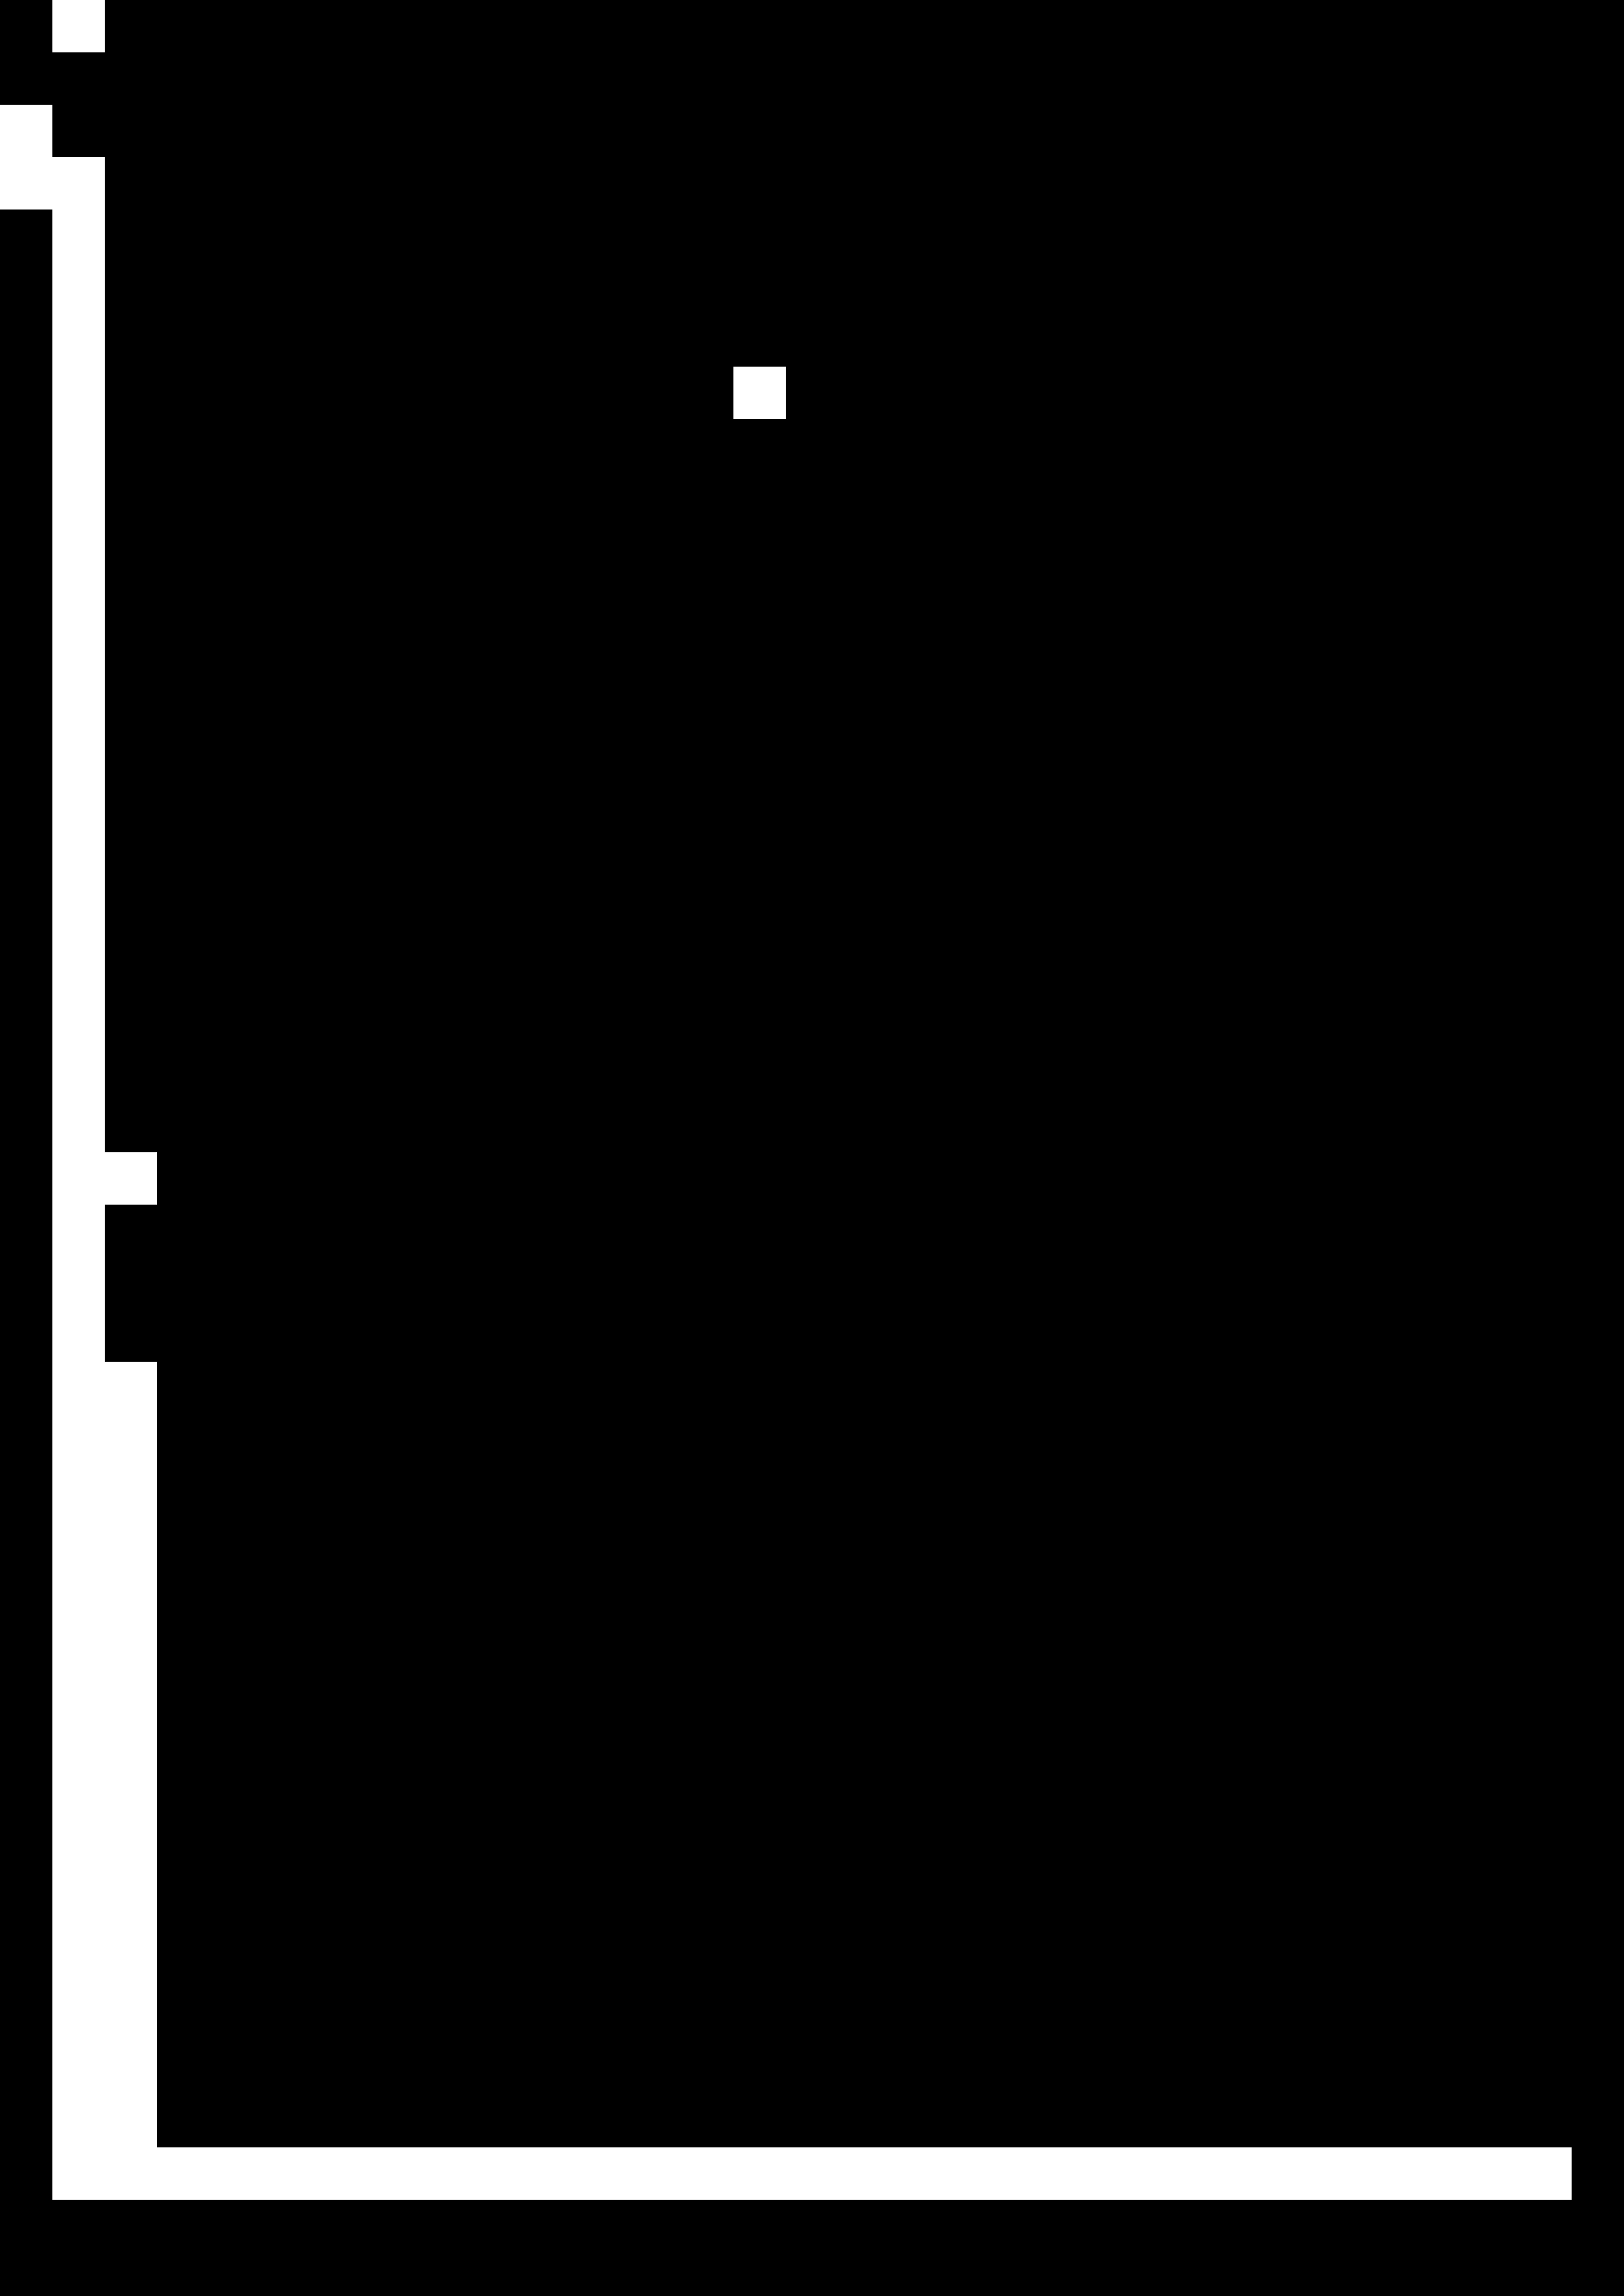
\includegraphics[scale=0.2]{images/1g_seuil.jpg}
\end{center}
\caption{seuillage puis attribution de la classe $fond$ (voisinage de taille 80 pixels)}
\label{seuillage}
\end{figure}

Reste à definir une classe ($texte$ ou $illustration$) aux pixels restants.

\section{Extraction de contours pour le texte}

Les contours au voisinage d'un pixel, semblent être une information pertinente pour caractériser les caractères d'un document numérisé.\\
En effet, les caractères sont généralement d'une couleur uniforme sur un fond uniforme (pour plus de lisiblité), ce qui a la 
particularité de bien faire ressortir les gradients\\
Pour extraire cette information, deux méthodes seront utilisées : l'application d'un filtre Laplacien et le calcul de l'histogramme orienté du gradient 
\cite{Dalal05histogramsof}, cela sur un patch carré. 

\section{Extraction de saturation pour les illustrations}

Comme évoqué precedemment, l'extraction d'une caractéristique de couleur est utile pour isoler les pixels d'illustration.\\
Utiliser le triplet RGB du voisinage d'un pixel n'a que peu de sens si on cherche à discriminer des pixels de texte (souvent noir).
En effet, le triplet HSV est plus approprié dans ce contexte : la saturation en particulier pour différencier les images couleur du texte gris-noir.\\
Les histogrammes des figures \ref{histo_hsv_illustration} et \ref{histo_hsv_texte} montrent parfaitement cette propriété : les patchs de texte ont des saturations
proches de 0, contrairement aux patchs d'illustration.\\

\begin{figure}[H]
\begin{center}
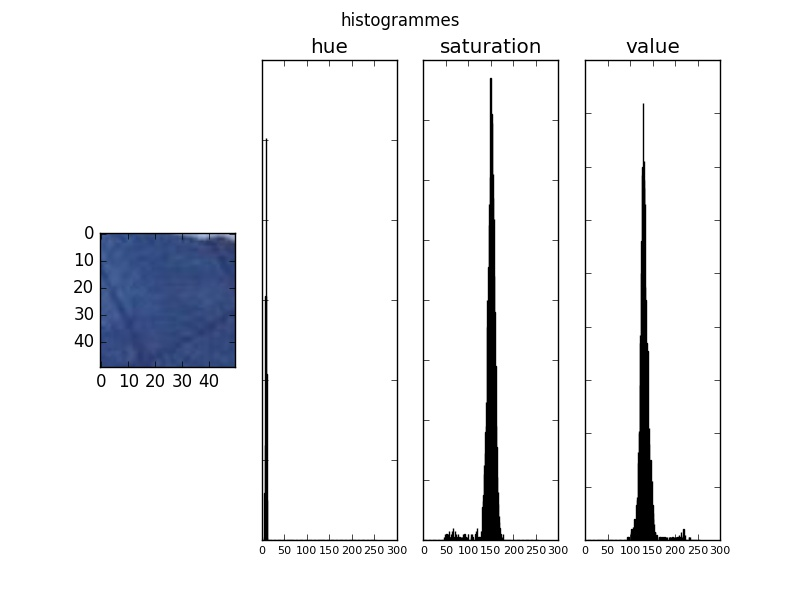
\includegraphics[scale=0.4]{images/histo_hsv_image.jpg}
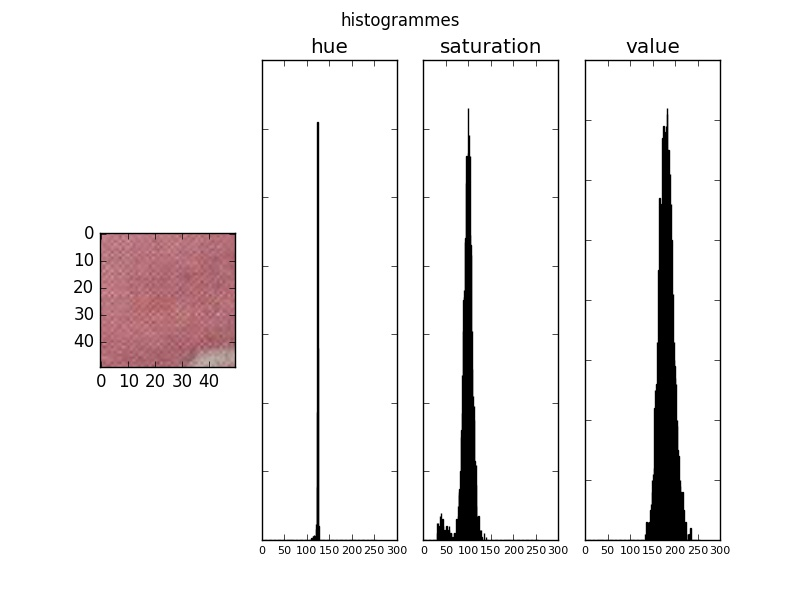
\includegraphics[scale=0.4]{images/histo_hsv_image2.jpg}
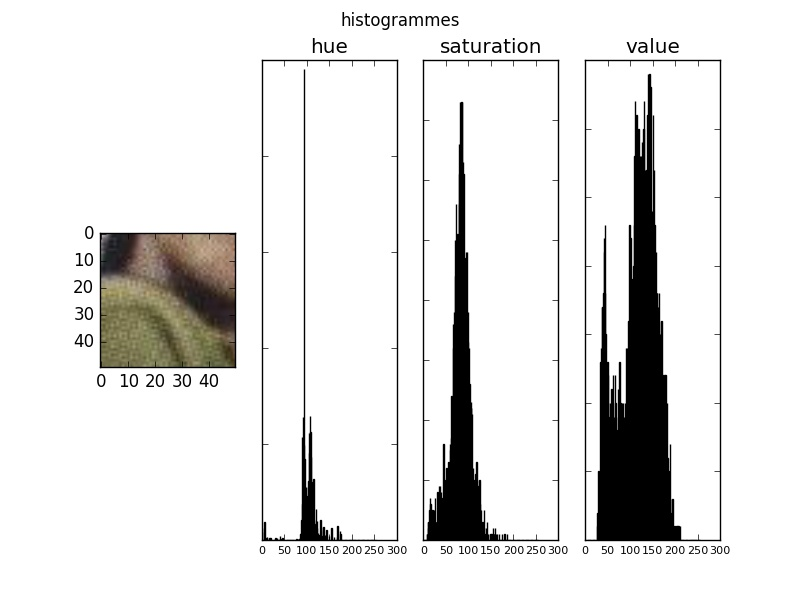
\includegraphics[scale=0.4]{images/histo_hsv_image3.jpg}
\end{center}
\caption{histogrammes HSV pour trois patchs d'illustration}
\label{histo_hsv_illustration}
\end{figure}

\begin{figure}[H]
\begin{center}
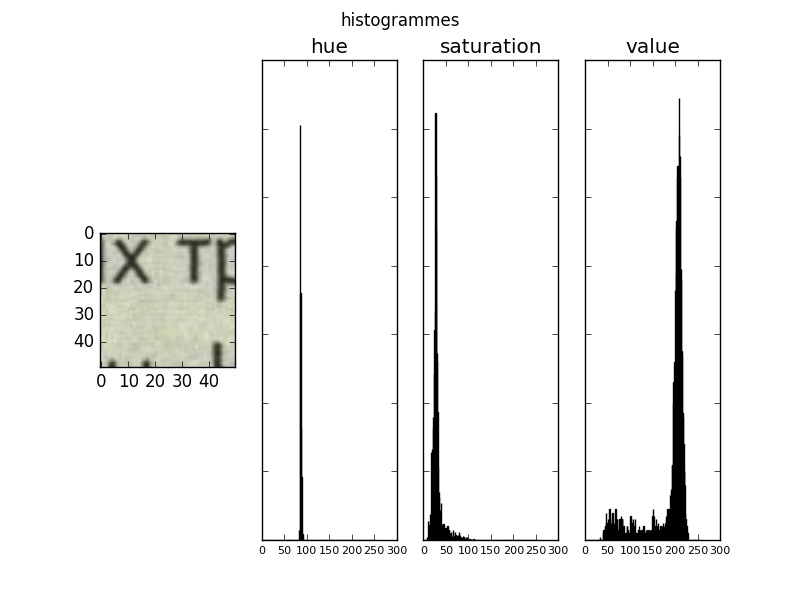
\includegraphics[scale=0.4]{images/histo_hsv_texte.jpg}
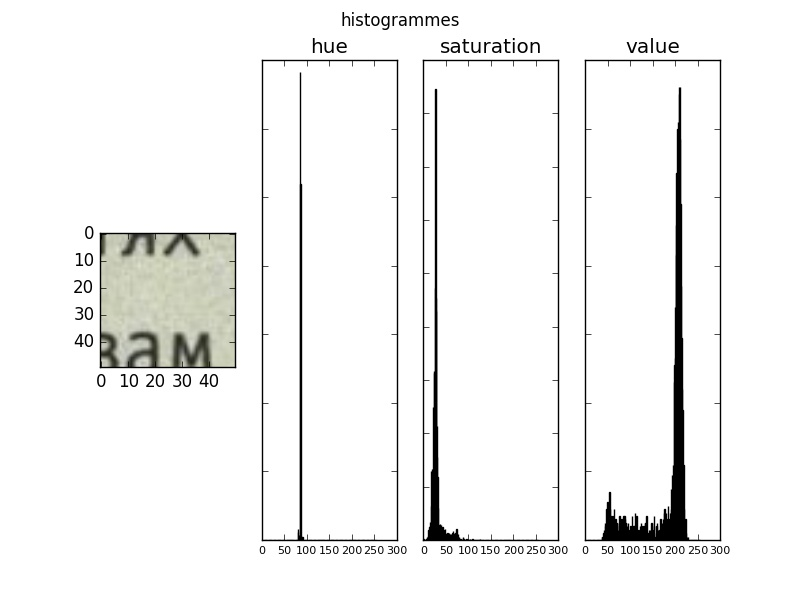
\includegraphics[scale=0.4]{images/histo_hsv_texte2.jpg}
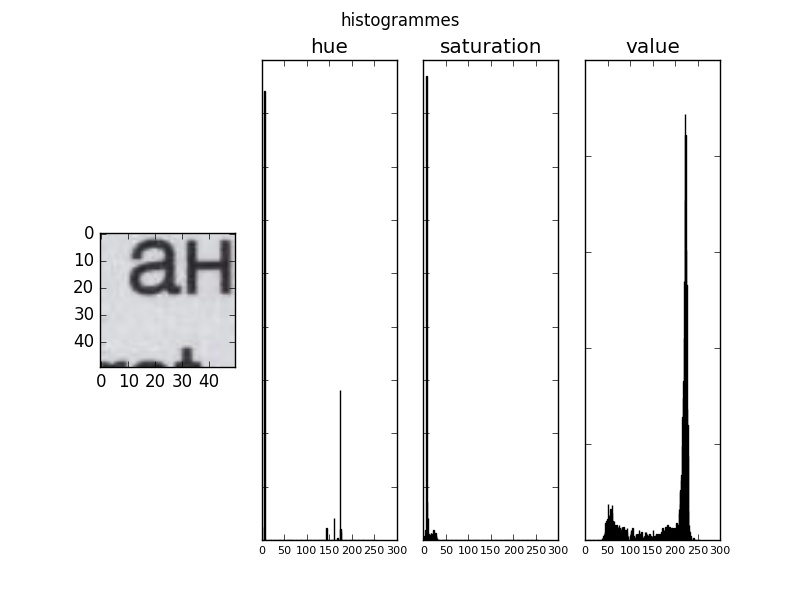
\includegraphics[scale=0.4]{images/histo_hsv_texte3.jpg}
\end{center}
\caption{histogrammes HSV pour trois patchs de texte}
\label{histo_hsv_texte}
\end{figure}


\chapter{Clustering}

A ce stade, nous avons des pixels qui ne sont pas du $fond$ et auxquels nous devons attribuer une classe parmi $texte$ et $illustration$.
Les features extraits au chapître précédents doivent donc être décomposer en deux sous groupes, à cet effet deux algorithmes sont utilisés :
\begin{description} % listes descriptives

\item[$KMeans$ :] cet algorithme permet de créer deux amas compactes par minimisation de l'énergie intra-cluster.
\item[$NMF$ :] cet algorithme permet de projeter les features des N pixels. Ces features de dimension P seront projetés sur un espace à 2 dimensions. On crééra ensuite
deux amas : un premier pour les points dont la première composante de projection est plus grande que la seconde, un second pour les autres.

\end{description}

A l'issue de cette étape de classification, nous avons donc deux amas de pixels. Nous définirons comme $texte$, l'amas de pixels dont la proportion de pixels blancs
est la plus grande. En effet, le texte possède plus de pixels blancs vu qu'il est très souvent écris sur fond blanc.\\
La figure \ref{resultat} montre l'application du $KMeans$ sur les descripteurs $HOG$+$HSV$ pour les pixels restants à déterminer.

\begin{figure}[H]
\begin{center}
%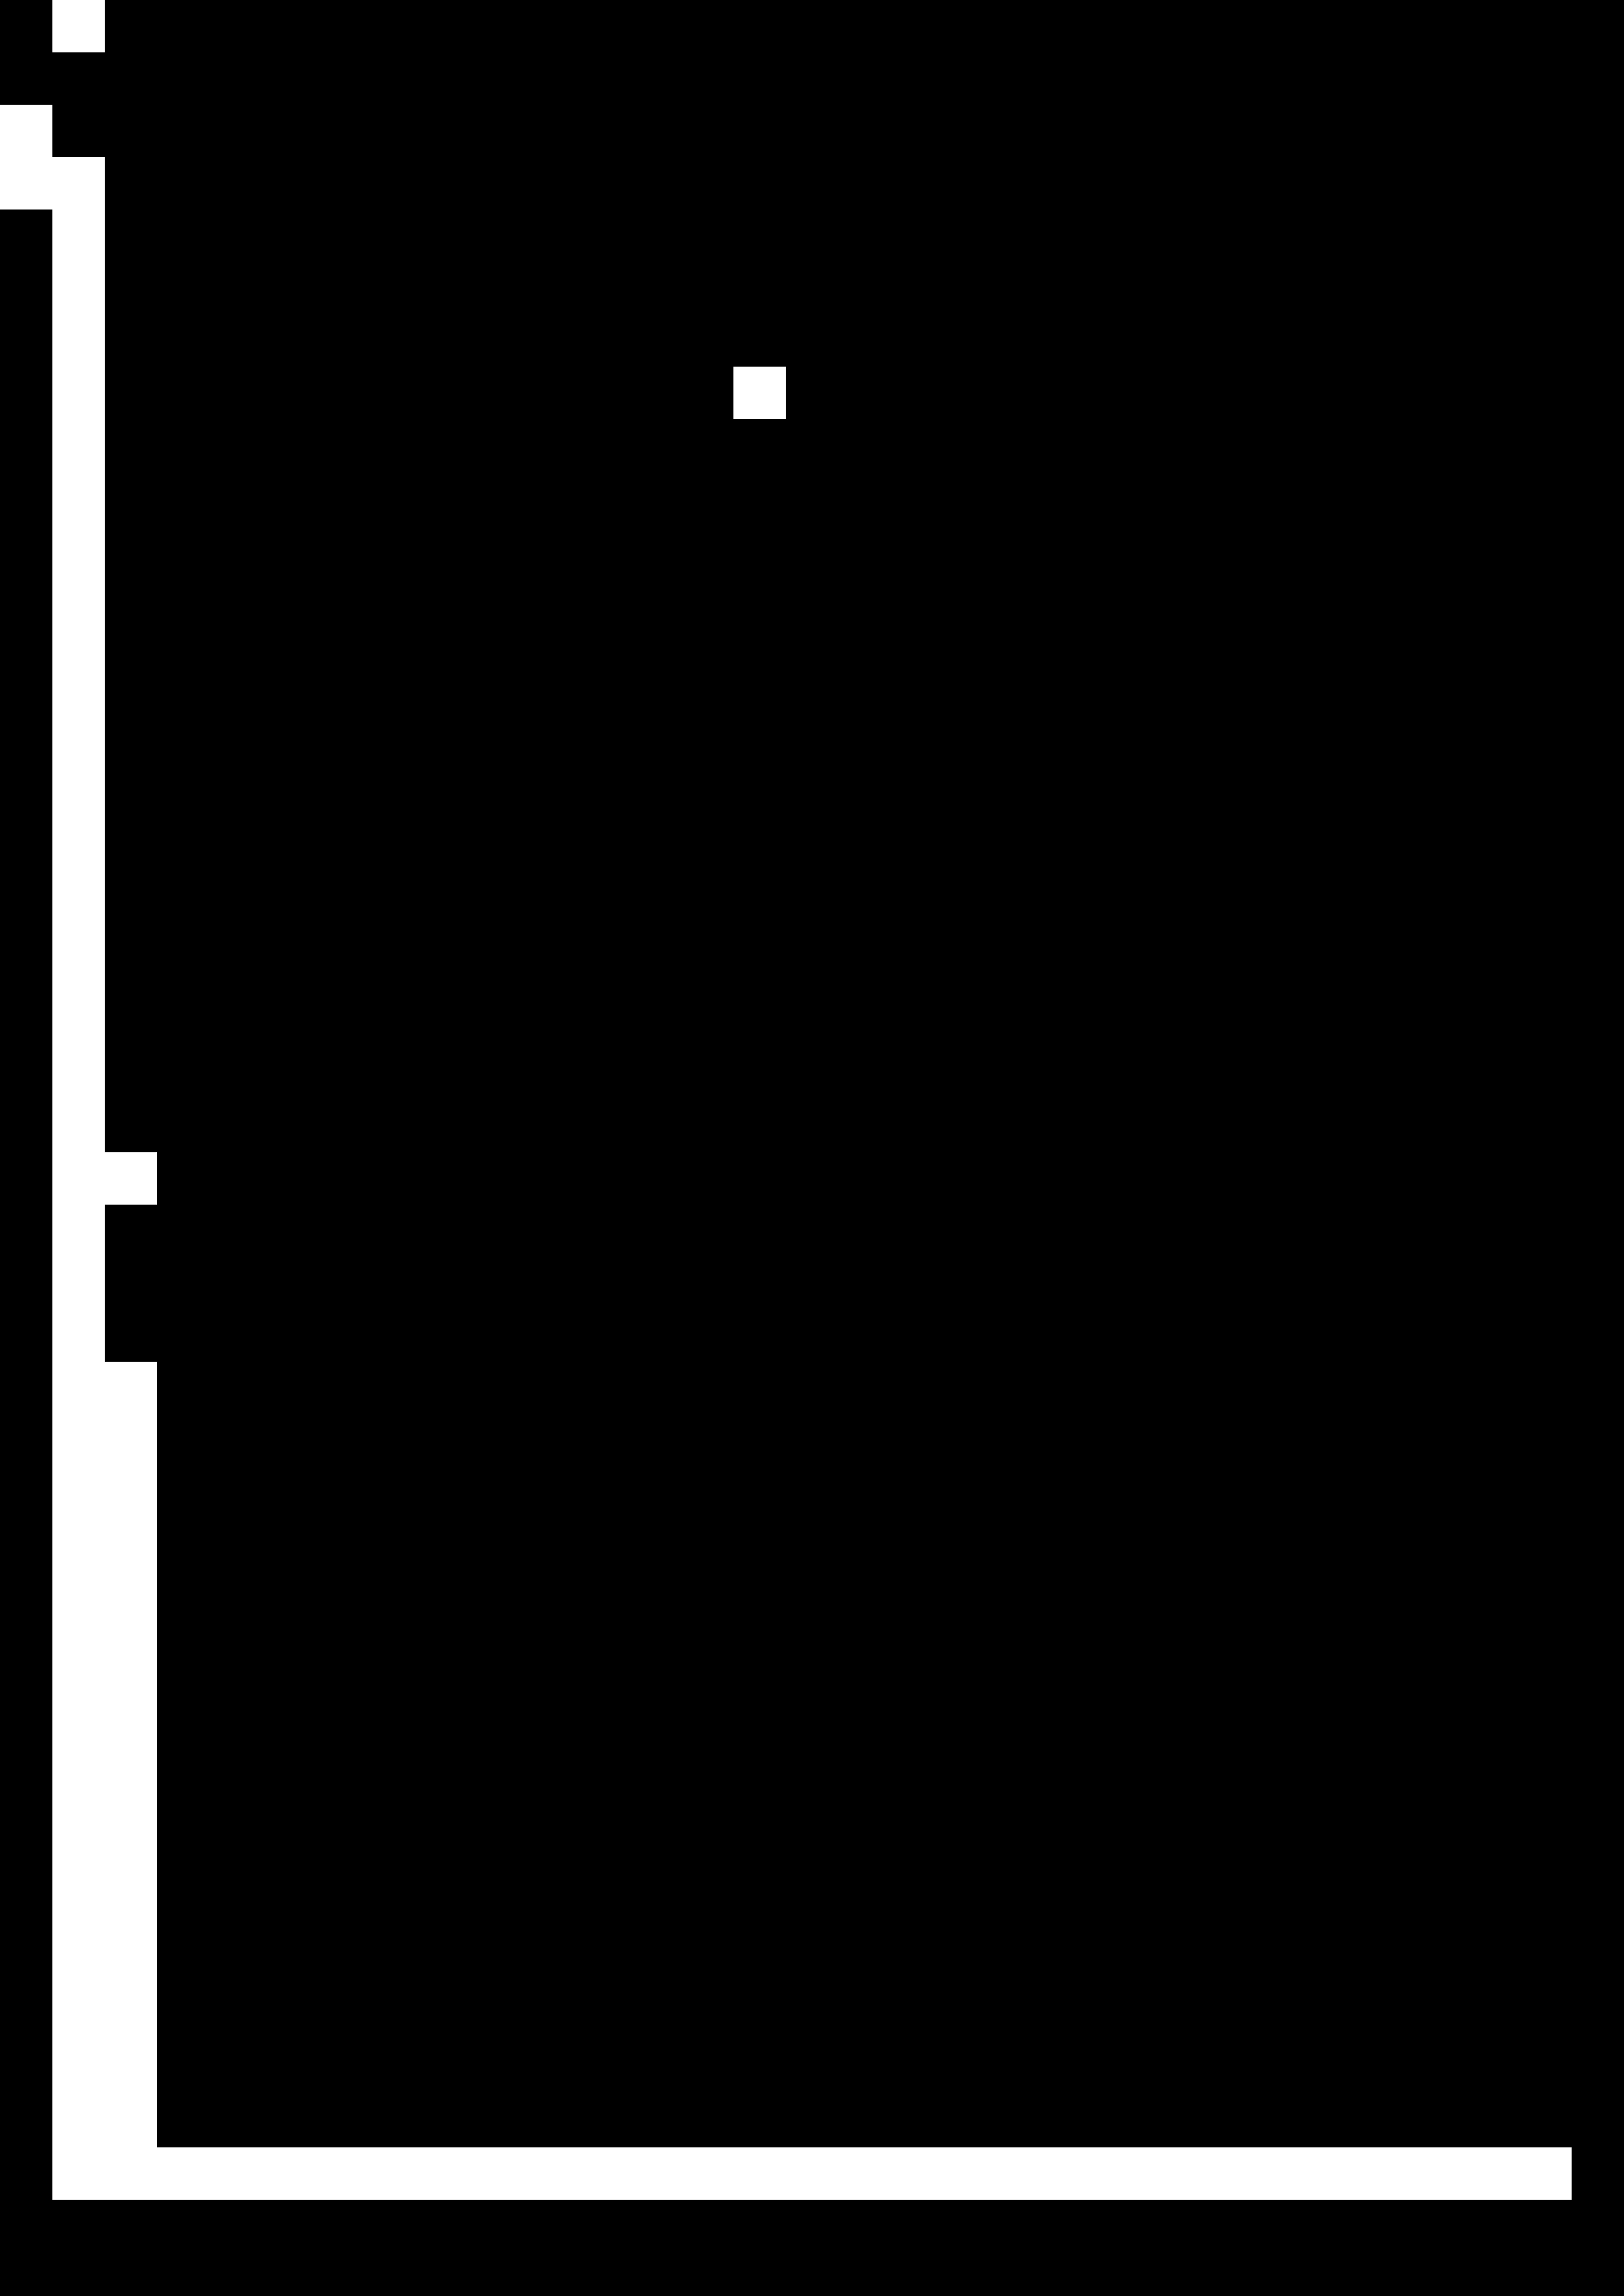
\includegraphics[scale=0.2]{images/1g_seuil.jpg}
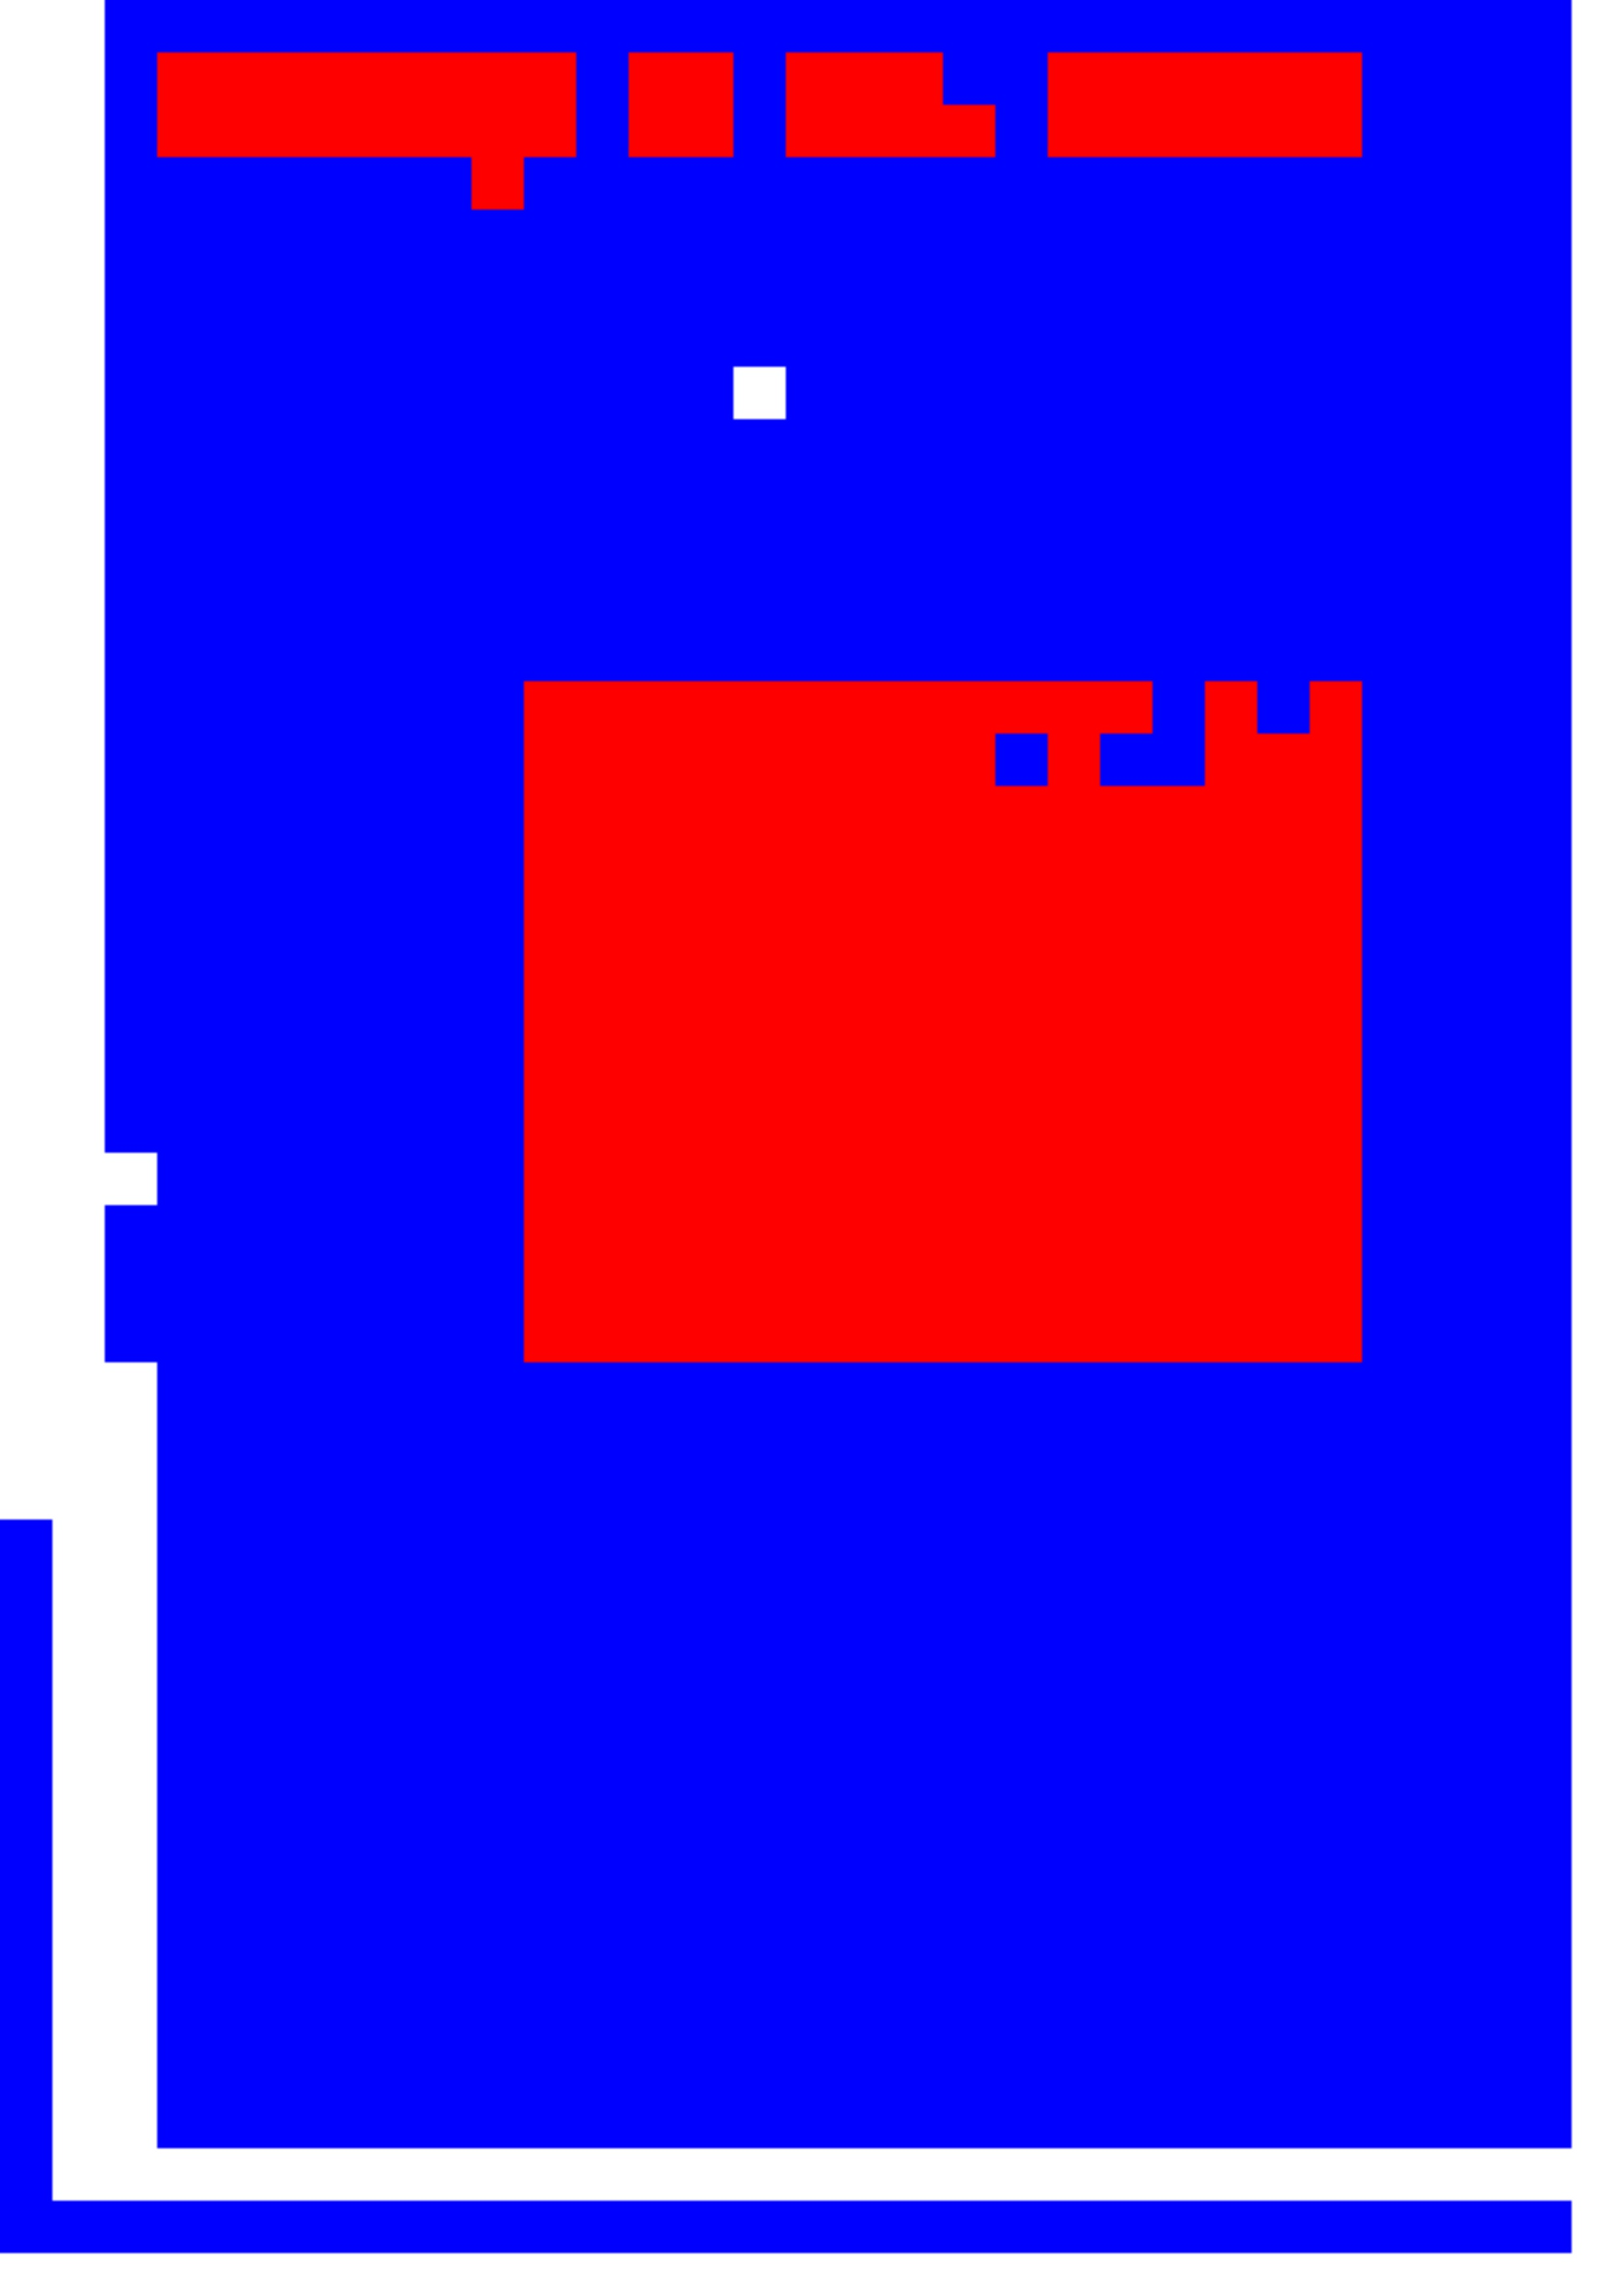
\includegraphics[scale=0.2]{images/1g_res_hog_hsv.jpg}
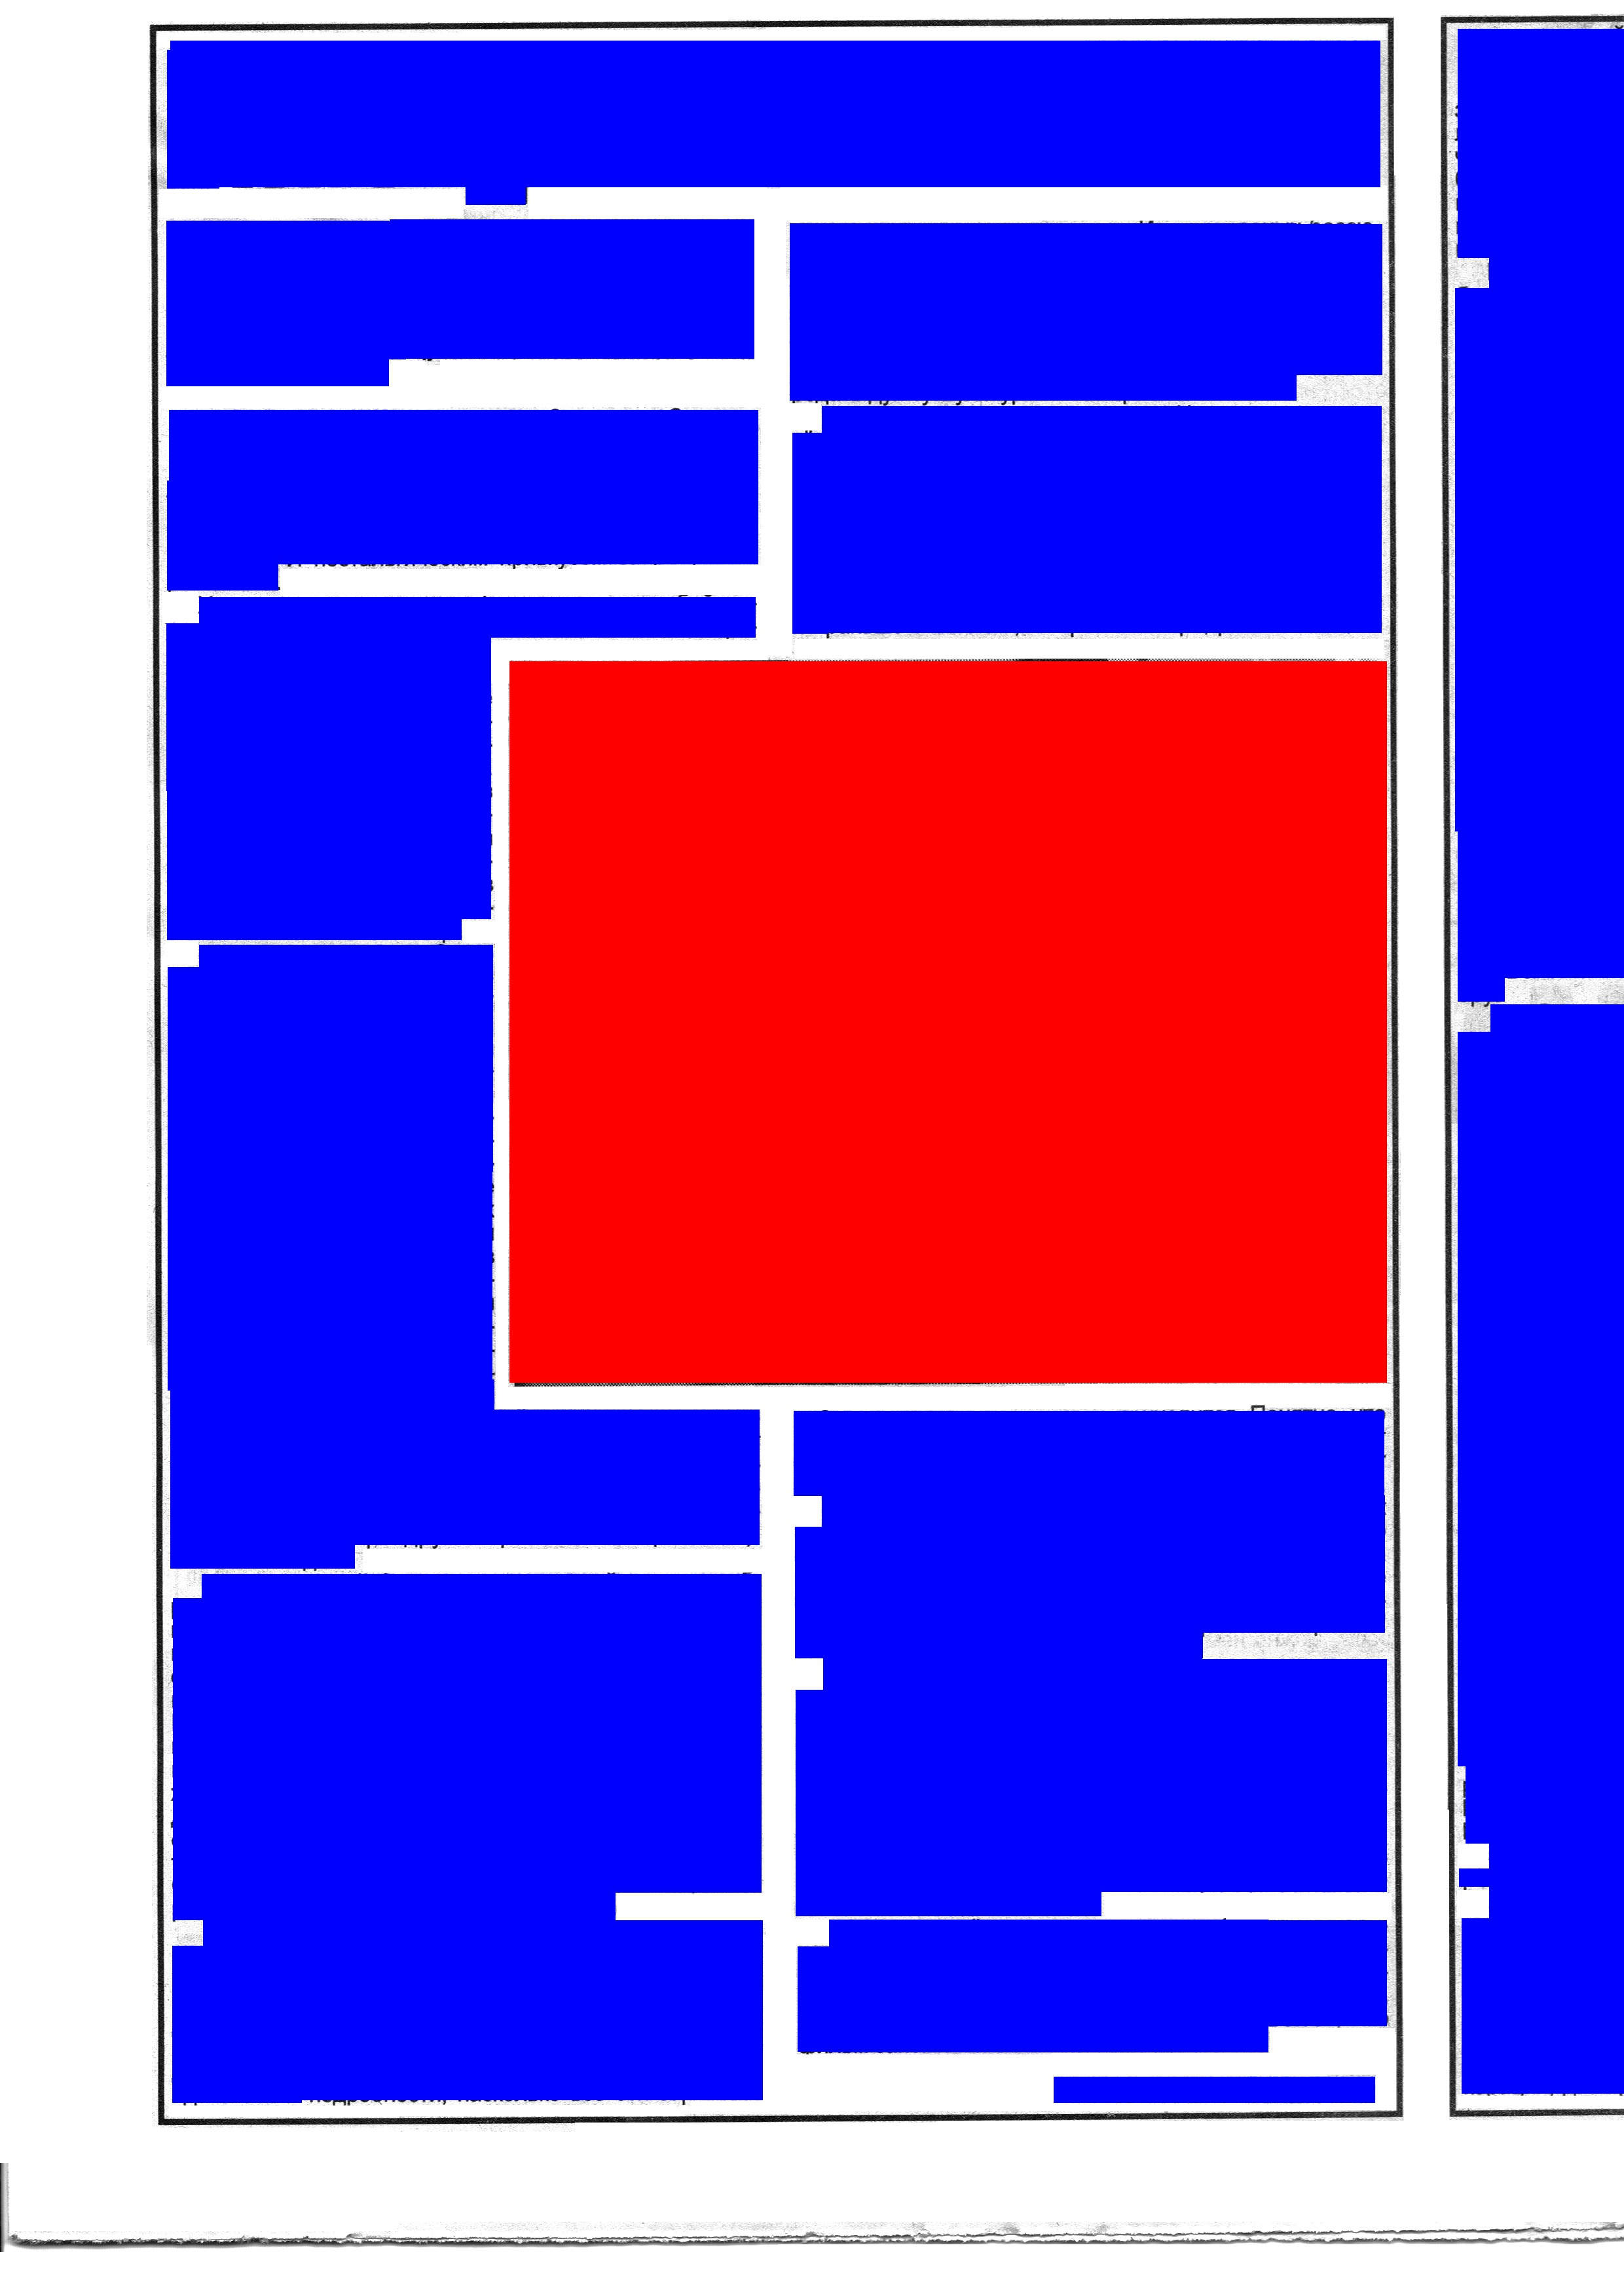
\includegraphics[scale=0.2]{images/1g_m.jpg}
\end{center}
\caption{seuillage puis attribution de la classe $fond$ (voisinage de taille 80 pixels) - vérité terrain}
\label{resultat}
\end{figure}


\chapter{Performances}

% \section{Précision/Rappel}

On applique le processus à toutes les images en procédant comme détaillé plus haut :

\begin{description}
 \item[-] Seuillage afin de déterminer les pixels de classe $fond$
 \item[-] Extraction de features des pixels restants (pour chaque pixel, concaténation du vecteur descripteurs HOG (ou Laplacien) et du vecteur descripteur HSV)
 \item[-] Clusterisation des features afin de déterminer la classe $illustration$ ou $texte$ des pixels restants
\end{description}

A des fins de mesures des performances, on utilise la vérité-terrain pour le calcul de précision/rappel pour chaque classe.\\
\ref{res_classe1},\ref{res_classe2} et \ref{res_classe3} récapitulent les precision/rappel obtenus respectivement pour les classes $fond$,$texte$ et $illustration$.

\begin{table}
\begin{center}
%\begin{tabular}{|p{5cm}|p{2cm}|p{2cm}|p{2cm}|p{2cm}|}
\begin{tabular}{|c|c|c|c|c|}
\hline
\multirow{\begin{bf}Descripteurs\end{bf}} & \multicolumn{2}{c|}{\begin{bf}KMeans\end{bf}} & \multicolumn{2}{c|}{\begin{bf}NMF\end{bf}}\\
\cline{2-5} & \begin{bf}precision\end{bf} & \begin{bf}recall\end{bf} & \begin{bf}precision\end{bf} & \begin{bf}recall\end{bf}\\
\hline
$Laplacien+HSV$ & 0.55 & 0.90 & 0.57 & 0.64\\
\hline
$HOG+HSV$ &  0.55 & 0.90 & 0.61 & 0.69\\
\hline
\end{tabular}
\end{center}
\caption{precision/rappel pour la classe $fond$}
\label{res_classe1}
\end{table}

\begin{table}
\begin{center}
%\begin{tabular}{|p{5cm}|p{2cm}|p{2cm}|p{2cm}|p{2cm}|}
\begin{tabular}{|c|c|c|c|c|}
\hline
\multirow{\begin{bf}Descripteurs\end{bf}} & \multicolumn{2}{c|}{\begin{bf}KMeans\end{bf}} & \multicolumn{2}{c|}{\begin{bf}NMF\end{bf}}\\
\cline{2-5} & \begin{bf}precision\end{bf} & \begin{bf}recall\end{bf} & \begin{bf}precision\end{bf} & \begin{bf}recall\end{bf}\\
\hline
$Laplacien+HSV$ & 0.63 & 0.55 & 0.38 & 0.40\\
\hline
$HOG+HSV$ &  0.64 & 0.61 & 0.39 & 0.47\\
\hline
\end{tabular}
\end{center}
\caption{precision/rappel pour la classe $illustration$}
\label{res_classe2}
\end{table}

\begin{table}
\begin{center}
%\begin{tabular}{|p{5cm}|p{2cm}|p{2cm}|p{2cm}|p{2cm}|}
\begin{tabular}{|c|c|c|c|c|}
\hline
\multirow{\begin{bf}Descripteurs\end{bf}} & \multicolumn{2}{c|}{\begin{bf}KMeans\end{bf}} & \multicolumn{2}{c|}{\begin{bf}NMF\end{bf}}\\
\cline{2-5} & \begin{bf}precision\end{bf} & \begin{bf}recall\end{bf} & \begin{bf}precision\end{bf} & \begin{bf}recall\end{bf}\\
\hline
$Laplacien+HSV$ & 0.83 & 0.65 & 0.53 & 0.58\\
\hline
$HOG+HSV$ & 0.87 & 0.66 & 0.75 & 0.62\\
\hline
\end{tabular}
\end{center}
\caption{precision/rappel pour la classe $texte$}
\label{res_classe3}
\end{table}

\clearpage

On oberve les meilleurs résultats pour un partitionnement $KMeans$ du descripteur $HOG+HSV$ avec une precision moyenne (toute image et toute classe confondue) de 
\begin{bf}0.68\end{bf} et un rappel moyen de \begin{bf}0.72\end{bf}.

\section{Cas particuliers}

\chapter{Code}

\chapter{Resultats}

\clearpage

\appendix
\chapter{Code Python pour l'extraction de saturation et sa classification}\label{code_python_saturation}
\begin{verbatim}
import numpy as np
import cv2
import os
import matplotlib.pyplot as plt
import shutil
import pandas as pd

saturation = []
path='c:/tmp/images_debat/'
dirs = os.listdir(path)
file_valid='c:/tmp/labels.csv'
# This would print all the files and directories
for file in dirs:
    if file.endswith((".jpg")):
        colorImage = cv2.imread(path+file)
        #print ('Traitement du fichier : ',path+file)
        rows, cols, nbChannels = colorImage.shape

        b,g,r = cv2.split(colorImage)
        colorImage=cv2.merge([r,g,b])
        color = ('b','g','r')
        clorImageHSV=cv2.cvtColor(colorImage, cv2.COLOR_BGR2HSV)
        h,s,v=cv2.split(clorImageHSV)
        sm=np.mean(s)
        saturation.append(sm)
        #if file == '00000108.jpg' or file == '00000110.jpg' or file == '00000147.jpg':
            #print ('saturation pour le fichier 108 - 110 -147:')
            #print sm

globalMean = np.mean(saturation)
print ('Moyenne globale:')
print globalMean
#print saturation
plt.hist(saturation, range = (35, 85), bins = 30, color = 'yellow',
            edgecolor = 'red')
plt.xlabel('Moyenne de la saturation')
plt.ylabel('nombre images')
plt.title('Histogramme saturation')
#hist=np.histogram(saturation)
#plt.bar(hist)
plt.show()
copyPathGrosPlan='c:/tmp/GrosPlan/'
copyPathLargePlan='c:/tmp/LargePlan/'
classif=pd.DataFrame(columns=('file_name', 'label'))
classif_multi=pd.DataFrame(columns=('file_name', 'sm'))
line = 0;
for file1 in dirs:
    if file1.endswith((".jpg")):
        colorImage = cv2.imread(path+file1)
        rows, cols, nbChannels = colorImage.shape

        r,g,b = cv2.split(colorImage)
        colorImage=cv2.merge([r,g,b])
        color = ('b','g','r')
        clorImageHSV=cv2.cvtColor(colorImage, cv2.COLOR_BGR2HSV)
        h,s,v=cv2.split(clorImageHSV)
        sm=np.mean(s)
        classif_multi.loc[line]=(file1,sm)
        #Gros plan
        if  sm <= (globalMean):
             classif.loc[line]=(file1,-1.)            
        #Large plan
        else:
            classif.loc[line]=(file1,1.)            
        
        line = line+1

classif.sort_values(['file_name'])
#print classif            
#Open the labelled file
labelfile = open(file_valid)
label_img = pd.read_csv(labelfile,sep=';', names=['file_name', 'label'],header=0,dtype={'label': float})
label_img.sort_values(['file_name'])
#print label_img

correct_predict = pd.merge(classif, label_img, on=['file_name', 'label'], how='inner')
#print len(correct_predict)
#print len(label_img)
print ('Resultat :', (float(len(correct_predict))/float(len(label_img)))*100.)
#print classif_multi
#print label_img
label_img_mrg = pd.merge(classif_multi, label_img, on=['file_name'], how='inner')
label_img_mrg = label_img_mrg.drop('file_name', 1)
#print label_img_mrg
label_img_mrg.to_csv('C:\perso\TP\Son-Image\classif_multi.csv', sep=';', encoding='utf-8')
\end{verbatim}

\backmatter

\listoftables

\listoffigures

\bibliographystyle{alpha}
\bibliography{biblio}

\end{document}